%%%%%%%% ICML 2021 EXAMPLE LATEX SUBMISSION FILE %%%%%%%%%%%%%%%%%

\documentclass{article}

% Recommended, but optional, packages for figures and better typesetting:
\usepackage{microtype}
\usepackage{graphicx}
\usepackage{subfigure}
\usepackage{booktabs} % for professional tables

% hyperref makes hyperlinks in the resulting PDF.
% If your build breaks (sometimes temporarily if a hyperlink spans a page)
% please comment out the following usepackage line and replace
% \usepackage{icml2021} with \usepackage[nohyperref]{icml2021} above.
\usepackage{hyperref}

% Attempt to make hyperref and algorithmic work together better:
%\newcommand{\theHalgorithm}{\arabic{algorithm}}

% Use the following line for the initial blind version submitted for review:
\usepackage{icml2021}

\let\zz\[\let\zzz\]

% if you need to pass options to natbib, use, e.g.:
%     \PassOptionsToPackage{numbers, compress}{natbib}
% before loading neurips_2020

% ready for submission
% \usepackage{neurips_2020}

% to compile a preprint version, e.g., for submission to arXiv, add add the
% [preprint] option:
%     \usepackage[preprint]{neurips_2020}

% to compile a camera-ready version, add the [final] option, e.g.:
%     \usepackage[final]{neurips_2020}

% to avoid loading the natbib package, add option nonatbib:
\usepackage[utf8]{inputenc} % allow utf-8 input
\usepackage[T1]{fontenc}    % use 8-bit T1 fonts
\usepackage{hyperref}       % hyperlinks
\usepackage{url}            % simple URL typesetting
\usepackage{booktabs}       % professional-quality tables
\usepackage{amsfonts}       % blackboard math symbols
\usepackage{nicefrac}       % compact symbols for 1/2, etc.
\usepackage{microtype}      % microtypography
\usepackage{comment}

\makeatletter
\def\set@curr@file#1{%
  \begingroup
    \escapechar\m@ne
    \xdef\@curr@file{\expandafter\string\csname #1\endcsname}%
  \endgroup
}
\def\quote@name#1{"\quote@@name#1\@gobble""}
\def\quote@@name#1"{#1\quote@@name}
\def\unquote@name#1{\quote@@name#1\@gobble"}
\makeatother
\usepackage{graphics}
\usepackage{microtype}
\usepackage{graphicx}
\usepackage{subfigure}
\usepackage{enumitem}
\usepackage{bm}
\usepackage{bbm}
\usepackage{booktabs} % for professional tables
% hyperref makes hyperlinks in the resulting PDF.
% If your build breaks (sometimes temporarily if a hyperlink spans a page)
% please comment out the following usepackage line and replace
% \usepackage{icml2019} with \usepackage[nohyperref]{icml2019} above.
%\usepackage{hyperref}


%\usepackage[textwidth=4cm,textsize=footnotesize]{todonotes}
\usepackage[disable]{todonotes}


%% our packages
\usepackage{mathtools}
\usepackage{amsmath,amssymb, amsthm}
\usepackage[nottoc]{tocbibind}
\usepackage{easyeqn}
\usepackage{xargs}
\usepackage{upgreek}
\usepackage{ifthen}
\usepackage{paracol}
\usepackage{url}
\usepackage{stmaryrd}

%\usepackage[numbers]{natbib}
% Attempt to make hyperref and algorithmic work together better:
%\newcommand{\theHalgorithm}{\arabic{algorithm}}



%% Our definitions go here
%\newcommand{\todo}[1]{{\bf \color{red} (TODO) #1}}

\usepackage{aliascnt}
\usepackage{cleveref}


\let\[\zz\let\]\zzz

\usepackage{amsthm}

\makeatletter
\newtheorem{theorem}{Theorem}
\crefname{theorem}{theorem}{Theorems}
\Crefname{Theorem}{Theorem}{Theorems}


\newaliascnt{proposition}{theorem}
\newtheorem{proposition}[proposition]{Proposition}
\aliascntresetthe{proposition}
\crefname{proposition}{proposition}{propositions}
\Crefname{Proposition}{Proposition}{Propositions}

\newaliascnt{lemma}{theorem}
\newtheorem{lemma}[lemma]{Lemma}
\aliascntresetthe{lemma}
\crefname{lemma}{lemma}{lemmas}
\Crefname{Lemma}{Lemma}{Lemmas}

\newaliascnt{corollary}{theorem}
\newtheorem{corollary}[corollary]{Corollary}
\aliascntresetthe{corollary}
\crefname{corollary}{corollary}{corollaries}
\Crefname{Corollary}{Corollary}{Corollaries}

\newtheorem{definition}{Definition}
\crefname{definition}{definition}{definitions}
\Crefname{Definition}{Definition}{Definitions}

\newtheorem{remark}{Remark}
\crefname{remark}{remark}{remarks}
\Crefname{Remark}{Remark}{Remarks}


\newtheorem{assumption}{\textbf{H}\hspace{-3pt}}
\Crefname{assumption}{\textbf{H}\hspace{-3pt}}{\textbf{H}\hspace{-3pt}}
\crefname{assumption}{\textbf{H}}{\textbf{H}}


 \def\elboneq{\mathcal{L}_{\IFIS}}

 \def\flow{\mathbf{T}}
\def\Cat{\operatorname{Cat}}

 \def\mass{\mathrm{M}}
 \def\Normal{\mathrm{N}}

  \providecommand{\assumptionname}{Assumption}
  \providecommand{\corollaryname}{Corollary}
  \providecommand{\lemmaname}{Lemma}
  \providecommand{\propositionname}{Proposition}
  \providecommand{\remarkname}{Remark}
\providecommand{\theoremname}{Theorem}

%\usepackage[disable]{todonotes}

\def\plaw{\operatorname{g}}

\def\simiid{\overset{\operatorname{iid}}{\sim}}
%% math commands go here
\def\IFIS{\ensuremath{\operatorname{InFiNE}}}
\def\InFiNE{{\small \IFIS}}
\def\MC{\mathrm{MC}}
\def\transfo{\operatorname{T}}
\def\dmid{\left.\middle\|\right.}
\def\rmd{\operatorname{d}\hspace{-2pt}}
\def\Id{\operatorname{Id}}
\def\PP{\mathbb{P}}
\def\QQ{\mathbb{Q}}
\def\PE{\mathbb{E}}
\def\PVar{\mathrm{Var}}
\def\mcf{\mathcal{F}}
\def\iid{i.i.d.}
\def\Ind{\mathbb{I}}
\def\ELBO{\operatorname{ELBO}}
\def\rset{\mathbb{R}}
\def\brset{\overline{\mathbb{R}}}
\def\nset{\mathbb{N}}
\def\nsets{\mathbb{N}^*}
\def\Ber{\mathrm{Ber}}
\def\dummy{f}
\def\nmeasrho{\tilde{\measrho}}

\newcommandx{\marginal}[2][1=]{\xi^{#2}_{#1}}

\newcommandx{\margindensm}[2]{m_{#1}^{#2}}
\newcommandx{\margindensmu}[4]{m_{#1}^{#2}(#3|#4)}


\newcommandx{\margindens}[4][4=]{\ifthenelse{\equal{#3}{}}{q_{#1}^{#4}(#2)}{q_{#1,#3}^{#4}(#2)}}
\newcommandx{\margindensw}[3][3=]{\ifthenelse{\equal{#3}{}}{q_{#1}^{#2}}{q_{#1,#3}^{#2}}}
\newcommand{\Mtrans}[4]{Q_{#1,#4}(#2,#3)}
\newcommand{\Mtransw}[2]{Q_{#1,#2}}
\newcommand{\chunk}[3]{#1_{#2:#3}}
\newcommand{\KL}[2]{\operatorname{KL}\left(#1\Vert #2\right)}
\newcommand{\KLLigne}[2]{\operatorname{KL}(#1| #2)}
\def\lowerbound{\mathcal{L}}
\def\lowerboundaux{\mathcal{L}_{\mathrm{aux}}}
\def\tlowerboundaux{\tilde{\mathcal{L}}_{\mathrm{aux}}}
\def\rmd{\mathrm{d}}
\def\bigO{\mathcal{O}}
\def\eqsp{\,}

\def\fwdtransfo{T}
\newcommandx{\fwdtransfoparam}[2]{\fwdtransfo_{#1,#2}}
\def\famtransfo{\mathcal{T}}
\def\invtransfo{\mathring{\fwdtransfo}}
\def\trueflow{\mathsf{T}}

\def\dmhratio{\mathring{\alpha}_{\phi,\tu}}
\def\counting{\mathsf{c}}

\def\msa{\mathsf{A}}
\def\borel{\mathcal{B}}
\newcommand{\defeq}{\vcentcolon=}
\newcommand{\eqdef}{=\vcentcolon}

\def\dimE{M}
\def\dimS{D}


\def\eg{\text{e.g.}}



\def\rmb{\mathrm{b}}

\def\mcu{\mathcal{U}}
\def\wrt{w.r.t.}

\def\phibf{\pmb{\phi}}
\def\bfphi{\phibf}

% Operands
\newcommand{\absolute}[1]{\left\vert #1 \right\vert}
\newcommand{\abs}[1]{\left\vert #1 \right\vert}
\newcommand{\absLigne}[1]{\vert #1 \vert}
\newcommand{\tvnorm}[1]{\| #1 \|_{\mathrm{TV}}}
\newcommand{\tvnormEq}[1]{\left \| #1 \right \|_{\mathrm{TV}}}
\newcommandx{\Vnorm}[2][1=V]{\| #2 \|_{#1}}
\newcommandx{\VnormEq}[2][1=V]{\ensuremath{\left\| #2 \right\|_{#1}}}
% \newcommandx{\norm}[2][1=]{\ifthenelse{\equal{#1}{}}{\left\Vert #2 \right\Vert}{\left\Vert #2 \right\Vert^{#1}}}
% \newcommandx{\normLigne}[2][1=]{\ifthenelse{\equal{#1}{}}{\Vert #2 \Vert}{\Vert #2\Vert^{#1}}}
\newcommand{\crochet}[1]{\left\langle#1 \right\rangle}
\newcommand{\parenthese}[1]{\left(#1 \right)}
\newcommand{\parentheseLigne}[1]{(#1 )}
\newcommand{\parentheseDeux}[1]{\left[ #1 \right]}
\newcommand{\parentheseDeuxLigne}[1]{[ #1 ]}
\newcommand{\defEns}[1]{\left\lbrace #1 \right\rbrace }
\newcommand{\defEnsLigne}[1]{\lbrace #1 \rbrace }
\newcommand{\defEnsPoint}[1]{\left\lbrace #1 \right. }
\newcommand{\defEnsPointDeux}[1]{\left. #1 \right  \rbrace }
\newcommand{\defEnsL}[1]{\left\lbrace #1 \right. }
\newcommand{\defEnsR}[1]{\left. #1 \right  \rbrace }

%\newcommand{\defSystem}[1]{\left\lbrace #1 \right. }

\newcommand{\ps}[2]{\left\langle#1,#2 \right\rangle}
\newcommand{\psLigne}[2]{\langle#1,#2 \rangle}

% Relations
\newcommand{\divid}{\mid}
\newcommand{\ndivide}{\nmid}

% Proba
\newcommand{\proba}[1]{\mathbb{P}\left( #1 \right)}
\newcommand{\probaCond}[2]{\mathbb{P}\left( \left. #1  \middle\vert #2 \right.\right)}
\newcommand{\probaLigne}[1]{\mathbb{P}( #1 )}
\newcommandx\probaMarkovTilde[2][2=]
{\ifthenelse{\equal{#2}{}}{{\widetilde{\mathbb{P}}_{#1}}}{\widetilde{\mathbb{P}}_{#1}\left[ #2\right]}}
\newcommand{\probaMarkov}[2]{\mathbb{P}_{#1}\left[ #2\right]}
\newcommand{\expe}[1]{\PE \left[ #1 \right]}
\newcommand{\expeExpo}[2]{\PE^{#1} \left[ #2 \right]}
\newcommand{\expeLigne}[1]{\PE [ #1 ]}
\newcommand{\expeLine}[1]{\PE [ #1 ]}
\newcommand{\expeMarkov}[2]{\PE_{#1} \left[ #2 \right]}
\newcommand{\expeMarkovLigne}[2]{\PE_{#1} [ #2 ]}
\newcommand{\expeMarkovExpo}[3]{\PE_{#1}^{#2} \left[ #3 \right]}
\newcommand{\probaMarkovTildeDeux}[2]{\widetilde{\mathbb{P}}_{#1} \left[ #2 \right]}
\newcommand{\expeMarkovTilde}[2]{\widetilde{\PE}_{#1} \left[ #2 \right]}

% Environments

%\renewenvironment{proof}[1][{\textit{Proof:}}]{\begin{trivlist} \item[\em{\hskip \labelsep #1}]}{\ensuremath{\qed} \end{trivlist}}

%\renewenvironment{proof}[1][{\textit{Proof:}}]{\begin{trivlist} \item[\em{\hskip \labelsep #1}]}{\ensuremath{\qed} \end{trivlist}}



%fleche limite
\newcommand{\flecheLimite}{\underset{n\to+\infty}{\longrightarrow}}
\newcommand{\flecheLimiteOption}[2]{\underset{#1\to#2}{\longrightarrow}}
\newcommand{\flecheLimiteHaut}{\overset{n\to+\infty}{\longrightarrow}}


%notation infini
\newcommand{\plusinfty}{+\infty}

%notation egale
\newcommand{\egale}[1]{\ensuremath{\underset{#1}{=}}}

%plusieurs ligne indice
%\sum\limits_{\substack{i=0 \\ i \neq i_0}}^{n}{A_



\newcommand\numberthis{\addtocounter{equation}{1}\tag{\theequation}}


\newcommand{\hilbert}{\mathcal{H}}


\def\ie{\textit{i.e.}}
%\def\as{almost surely}
\def\cadlag{càdlàg}
\def\eqsp{\;}
\newcommand{\coint}[1]{\left[#1\right)}
\newcommand{\ocint}[1]{\left(#1\right]}
\newcommand{\ooint}[1]{\left(#1\right)}
\newcommand{\ccint}[1]{\left[#1\right]}
\newcommand{\cointLigne}[1]{[#1)}
\newcommand{\ocintLigne}[1]{(#1]}
\newcommand{\oointLigne}[1]{(#1)}
\newcommand{\ccintLigne}[1]{[#1]}
\renewcommand{\iint}[2]{\left\lbrace #1,\ldots,#2\right\rbrace}
\newcommand{\iintLigne}[2]{\lbrace #1,\ldots,#2\rbrace}


\def\primr{f_r}
\def\primrO{f_{r_0}}



\newcommand{\1}{\mathbbm{1}}
\newcommand{\indi}[1]{\1_{#1}}
\newcommand{\indiacc}[1]{\mathbbm{1}_{\{ #1   \}}}
\newcommandx{\weight}[2][2=n]{\omega_{#1,#2}^N}
\newcommand{\loi}{\mathcal{L}}
\newcommand{\boule}[2]{\operatorname{B}(#1,#2)}
\newcommand{\ball}[2]{\operatorname{B}(#1,#2)}
\newcommand{\boulefermee}[2]{\overline{\mathrm{B}}(#1,#2)}
\newcommand{\diameter}{\operatorname{diam}}
\newcommand{\deta}{d_{\eta}}

\def\TV{\mathrm{TV}}




 \newcommand{\alaini}[1]{\todo[color=black!20,inline]{{\bf AD:} #1}}
  \newcommand{\alain}[1]{\todo[color=black!20]{{\bf AD:} #1}}
 \newcommand{\tcr}[1]{\textcolor{red}{#1}}
% \newcommand{\tcb}[1]{\textcolor{blue}{#1}}
 \newcommand{\arnaud}[1]{\todo[color=red!20]{{\bf Arno:} #1}}
  \newcommand{\xian}[1]{\todo[color=orange!30]{{\bf Xian:} #1}}
  \newcommand{\achille}[1]{\todo[color=blue!30]{{\bf AT:} #1}}

\def\as{almost surely}
\def\dist{\operatorname{dist}}

\newcommandx\sequence[3][2=,3=]
{\ifthenelse{\equal{#3}{}}{\ensuremath{\{ #1_{#2}\}}}{\ensuremath{\{ #1_{#2}, \eqsp #2 \in #3 \}}}}
\newcommandx\sequenceD[3][2=,3=]
{\ifthenelse{\equal{#3}{}}{\ensuremath{\{ #1_{#2}\}}}{\ensuremath{( #1)_{ #2 \in #3} }}}

\newcommandx{\sequencen}[2][2=n\in\N]{\ensuremath{\{ #1_n, \eqsp #2 \}}}
\newcommandx\sequenceDouble[4][3=,4=]
{\ifthenelse{\equal{#3}{}}{\ensuremath{\{ (#1_{#3},#2_{#3}) \}}}{\ensuremath{\{  (#1_{#3},#2_{#3}), \eqsp #3 \in #4 \}}}}
\newcommandx{\sequencenDouble}[3][3=n\in\N]{\ensuremath{\{ (#1_{n},#2_{n}), \eqsp #3 \}}}


\def\iid{i.i.d.}
\def\ifof{if and only if}
\def\eg{e.g.}


\newcommand{\note}[1]{{\textbf{\color{red}#1}}}


\newcommand{\opnorm}[1]{{\left\vert\kern-0.25ex\left\vert\kern-0.25ex\left\vert #1
    \right\vert\kern-0.25ex\right\vert\kern-0.25ex\right\vert}}



\def\Lip{\operatorname{Lip}}
\def\generator{\mathcal{A}}
\def\generatorsp{\generator^{\sphere^d}}
\def\generatorr{\generator^{\rset^d}}

\def\momentNoise{\mathrm{m}}
\def\bfe{\mathbf{e}}

\def\bfv{\mathbf{v}}
\def\ebf{\mathbf{e}}
\def\vbf{\mathbf{v}}


\def\Id{\operatorname{Id}}

\def\tildetheta{\tilde{\theta}}

\def\calC{\mathcal{C}}

\def\varphibf{\operatorname{g}}
\newcommandx{\CPE}[3][1=]{{\mathbb E}_{#1}\left[\left. #2 \middle \vert #3 \right. \right]} %%%% esperance conditionnelle
\newcommandx{\CPVar}[3][1=]{\mathrm{Var}^{#3}_{#1}\left\{ #2 \right\}}
\newcommand{\CPP}[3][]
{\ifthenelse{\equal{#1}{}}{{\mathbb P}\left(\left. #2 \, \right| #3 \right)}{{\mathbb P}_{#1}\left(\left. #2 \, \right | #3 \right)}}

\def\Ascr{\mathscr{A}}
\def\scrA{\mathscr{A}}
\def\scrB{\mcbb}
\def\scrC{\mathscr{C}}

\def\barL{\bar{L}}

\def\YL{\mathbf{Y}}
\def\XEM{X}
\def\steps{\gamma}
\def\measSet{\mathbb{M}}

\newcommand\Ent[2]{\mathrm{Ent}_{#1}\left(#2\right)}
\newcommandx{\osc}[2][1=]{\mathrm{osc}_{#1}(#2)}

\def\Ybar{\bar{Y}}
\def\Id{\operatorname{Id}}
\def\IdM{\operatorname{I}_d}
\newcommand\EntDeux[2]{\Ent_{#1}\left[#2 \right]}
\def\Ltwo{\mathrm{L}^2}
\def\Lone{\mathrm{L}^1}
\newcommand\densityPi[1]{\frac{\rmd #1}{\rmd \pi}}
\newcommand\densityPiLigne[1]{\rmd #1 /\rmd \pi}
\newcommand\density[2]{\frac{\rmd #1}{\rmd #2}}
\newcommand\densityLigne[2]{\rmd #1/\rmd #2}

\def\V{V}
\def\VD{V}
\def\Vsp{V^{\sphere^d}_{\b,\beta}}
\def\Vr{V^{\rset^d}_{\b,\c,\beta}}

\def\Prset{P^{\rset^d}}
\def\Psphere{P^{\sphere^d}}

\def\n{\mathrm{n}}
\def\Vpsi{\psi}
\def\Vkappa{\kappa}
\def\Vkappat{\tilde{\kappa}}
\def\Vchi{\chi}
\def\Vchit{\tilde{\chi}}
\def\Vphi{\phi}
\def\Vrho{\rho}
\def\psiV{\Vpsi}
\def\rhoV{\Vrho}
\def\phiV{\Vphi}
\def\fV{f}
\def\Vf{\fV}
\def\kappaVt{\tilde{\Vkappa}}
\def\kappaV{\Vkappa}
\def\chiV{\Vchi}
\def\chiVt{\Vchit}


\def\a{a}
\def\b{b}
\def\c{c}
\def\e{e}
\def\rU{\mathrm{r}}

\def\domain{\mathrm{D}}

\def\martfg{M^{f,g}}
\newcommand\Ddir[1]{D_{#1}}
\newcommand\maxplus[1]{\parenthese{#1}_+}
\def\Refl{\mathrm{R}}
\def\phibf{\pmb{\phi}}
\def\Gammabf{\mathbf{\Gamma}}


\def\transpose{\operatorname{T}}
\def\v{v}
\def\w{w}
\def\y{y}
\def\z{z}
%%%% bar

\def\bb{\bar{b}}
\def\bgamma{\bar{\gamma}}
\def\bU{\bar{U}}
\def\Ub{\bU}
\def\lambdab{\bar{\lambda}}
\def\blambdab{\bar{\lambda}}
\def\bv{\bar{v}}
\def\vb{\bv}
\def\yb{\bar{y}}
\def\by{\yb}
\def\Xb{\bar{X}}
\def\Yb{\bar{Y}}
\def\Gb{\bar{G}}
\def\Eb{\bar{E}}
\def\Tb{\bar{T}}
\def\taub{\bar{\tau}}

\def\bX{\bar{X}}
\def\bY{\bar{Y}}
\def\bG{\bar{G}}
\def\bE{\bar{E}}
\def\bT{\bar{T}}
\def\btau{\bar{\tau}}

\def\pib{\bar{\pi}}
\def\bpi{\pib}

\def\S{S}
\def\target{\pi}
\def\proposal{\rho}
\def\weightfunc{\tilde{w}}
\newcommand{\chunku}[3]{#1^{#2:#3}}
\newcommand{\chunkl}[3]{#1_{#2:#3}}
\newcommand{\chunkul}[5]{#1_{#2:#3}^{#4:#5}}
\newcommand{\chunkum}[4]{#1^{#2:#3 \setminus \{#4\}}}
\newcommand{\chunkulm}[6]{#1_{#2:#3}^{#4:#5 \setminus \{#4\}}}
\def\ISIR{\operatorname{ISIR}}
%%%%
% \tilde

\def\tr{\tilde{r}}
\def\tc{\tilde{c}}
\def\tmsk{\tilde{\msk}}
\def\tW{\tilde{W}}
\def\tvarsigma{\tilde{\varsigma}}
\def\tv{\tilde{v}}
\def\vt{\tv}
\def\yt{\tilde{y}}
\def\ty{\yt}
\def\Mt{\tilde{M}}
\def\tM{\Mt}

\def\tx{\tilde{x}}
\def\xt{\tx}
\def\Xt{\tilde{X}}
\def\Yt{\tilde{Y}}
\def\Gt{\tilde{G}}
\def\Et{\tilde{E}}
\def\Tt{\tilde{T}}
\def\St{\tilde{S}}
\def\taut{\tilde{\tau}}

\def\tX{\tilde{X}}
\def\tY{\tilde{Y}}
\def\tG{\tilde{G}}
\def\tE{\tilde{E}}
\def\tT{\tilde{T}}
\def\tS{\tilde{S}}
\def\ttau{\tilde{\tau}}
\def\teta{\tilde{\eta}}
\newcommand{\ttheta}{\tilde{\theta}}


%%%%%
% \bar
\def\Xb{\bar{X}}
\def\Yb{\bar{Y}}
\def\Gb{\bar{G}}
\def\Eb{\bar{E}}
\def\Tb{\bar{T}}
\def\Sb{\bar{S}}
\def\taub{\bar{\tau}}
\def\Hb{\bar{H}}
\def\Nb{\bar{N}}


\def\bX{\bar{X}}
\def\bY{\bar{Y}}
\def\bG{\bar{G}}
\def\bE{\bar{E}}
\def\bT{\bar{T}}
\def\btau{\bar{\tau}}
\def\bS{\bar{S}}
\def\bH{\bar{H}}
\def\bN{\bar{N}}

%%%%%%%%

\def\mgU{\mathrm{m}_{\nabla U}}
\def\MintDrift{I}
\def\CU{C_U}
\def\RU{R_1}
\def\RV{R}
\def\Reps{R_{\epsilon}}
\def\Resp{\Reps}
\def\veps{\varepsilon}
\def\sphere{\mss}

\def\nablaUt{\overline{\nabla U}}
\def\measureSphere{\nu^d}

\def\etaU{\eta}
\def\epsilonU{\epsilon}

\def\Jac{\mathbf{J}}
\newcommand{\JacOp}[1]{\Jac_{#1}}
\def\jac{\operatorname{Jac}}
\def\sign{\operatorname{sign}}
\def\rate{\lambda_{\mathrm{r}}}
\newcommand{\intentier}[2]{[#1:#2]}
\newcommand{\intentierU}[1]{[#1]}
%\newcommand{\intentier}[2]{#1:#2}
\def\measrho{\boldsymbol{\rho}}
\def\rmi{\mathrm{I}}
\def\ne{\mathrm{ne}}
\def\const{Z}
\def\estConst{\widehat{Z}}
\newcommand{\estConstC}[1]{\widehat{Z}_{#1}}
\newcommand{\estConstCphi}[2]{\widehat{Z}_{#1}^{#2}}
\newcommand{\hatpi}[1]{\hat{\pi}_{#1}}
%\def\hatpi{\hat{\pi}}
\def\measpi{\boldsymbol{\pi}}
\def\measprop{\boldsymbol{\rho}}
\def\measq{\boldsymbol{q}}


\def\sigmaS{\sigma^2}

\newcommand{\ensemble}[2]{\left\{#1\,:\eqsp #2\right\}}
\newcommand{\ensembleLigne}[2]{\{#1\,:\eqsp #2\}}
\newcommand{\set}[2]{\ensemble{#1}{#2}}

\def\rmD{\mathrm{D}}%%rmd déjà pris
\def\mrd{\mathrm{D}}
\def\mrc{\mathrm{C}}

\def\diag{\Delta_{\rset^d}}

\def\lyap{V}
\newcommand\coupling[2]{\Gamma(\mu,\nu)}
\def\supp{\mathrm{supp}}
\def\tpi{\tilde{\pi}}
\newcommand\adh[1]{\overline{#1}}

\def\ACb{\mathrm{AC}_{\mathrm{b}}}

\def\opK{\mathrm{K}}

\newcommand{\fracm}[2]{\left. #1 \middle / #2 \right.}

\newcommand{\complementary}{\mathrm{c}}

\def\poty{H}
\def\diam{\mathrm{diam}}
\def\talpha{\tilde{\alpha}}
\def\Leb{\mathrm{Leb}}
\newcommand{\iintD}[2]{\{#1,\ldots,#2\}}
\def\interior{\mathrm{int}}
\def\iff{ if and only if }

\def\vareps{\varepsilon}
\def\varespilon{\varepsilon}
\def\si{\text{ if } }
\def\projd{\operatorname{proj}^{\msd}}
\def\Phibf{\mathbf{\Phi}}

\def\RKer{R_{\gamma}}

\def\VEa{V}
\def\KUa{K}
\def\vol{\operatorname{Vol}}

\newcommand*\Let[1]{\State #1 }

\def\mU{\mathrm{m}}

\newcommand\fraca[2]{(#1)/(#2)}

\def\ccur{\mathtt{c}}
\def\Ve{V_{\rme}}
\def\Rad{\operatorname{Rad}}
%%% mathsf
\def\msi{\mathsf{I}}
\def\msw{\mathsf{W}}
\def\msa{\mathsf{A}}
\def\msd{\mathsf{D}}
\def\msk{\mathsf{K}}
\def\mss{\mathsf{S}}
\def\msn{\mathsf{N}}
\def\msat{\tilde{\mathsf{A}}}
\def\msb{\mathsf{B}}
\def\msc{\mathsf{C}}
\def\mse{\mathsf{E}}
\def\msf{\mathsf{F}}
\def\mso{\mathsf{O}}
\def\msg{\mathsf{G}}
\def\msh{\mathsf{H}}
\def\msm{\mathsf{M}}
\def\msu{\mathsf{U}}
\def\tmsu{{\mathsf{U}}}
\def\msv{\mathsf{V}}
\def\msr{\mathsf{R}}
\newcommand{\msff}[2]{\mathsf{F}_{#1}^{#2}}
\def\msp{\mathsf{P}}
\def\msq{\mathsf{Q}}
\def\msx{\mathsf{X}}
\def\msy{\mathsf{Y}}

\def\msphi{\mathsf{\Phi}}

%% mathcal
\def\mca{\mathcal{A}}
\def\mcl{\mathcal{L}}
\def\mcat{\tilde{\mathcal{A}}}
\def\mcab{\bar{\mathcal{A}}}
\def\mcbb{\mathcal{B}}  %%% \mcb est déjà pris
\newcommand{\mcb}[1]{\mathcal{B}(#1)}
\def\mcc{\mathcal{C}}
\def\mcy{\mathcal{Y}}
\def\mcx{\mathcal{X}}
\def\mce{\mathcal{E}}
\def\mcf{\mathcal{F}}
\def\mcg{\mathcal{G}}
\def\mch{\mathcal{H}}
\def\mcm{\mathcal{M}}
\def\mcu{\mathcal{U}}
\def\mcv{\mathcal{V}}
\def\mcr{\mathcal{R}}
\newcommand{\mcff}[2]{\mathcal{F}_{#1}^{#2}}
\def\mcfb{\bar{\mathcal{F}}}
\def\bmcf{\bar{\mathcal{F}}}
\def\mcft{\tilde{\mathcal{F}}}
\def\tmcf{\tilde{\mathcal{F}}}
\def\mcp{\mathcal{P}}
\def\mcq{\mathcal{Q}}

%% mathbb

\def\rset{\mathbb{R}}
\def\rsets{\mathbb{R}^*}
\def\cset{\mathbb{C}}
\def\zset{\mathbb{Z}}
\def\nset{\mathbb{N}}
\def\nsets{\mathbb{N}^*}
\def\qset{\mathbb{Q}}
\def\Rset{\mathbb{R}}
\def\Cset{\mathbb{C}}
\def\Zset{\mathbb{Z}}
\def\Nset{\mathbb{N}}
\def\Tset{\mathbb{T}}


%%%% mathrm


\def\rmP{\mathrm{P}}
\def\rmQ{\mathrm{Q}}
\def\rml{\mathrm{L}}
\def\rmR{\mathrm{R}}
\def\rmS{\mathrm{S}}
\def\rmT{\mathrm{T}}
\def\rmM{\mathrm{M}}
\def\Prm{\mathrm{P}}
\def\rmb{\mathrm{b}}
\def\mrb{\mathrm{b}}
\def\rmd{\mathrm{d}}
\def\rmZ{\mathrm{Z}}
\def\mrd{\mathrm{d}}
\def\mre{\mathrm{e}}
\def\rme{\mathrm{e}}
\def\rmn{\mathrm{n}}
\def\mrn{\mathrm{n}}
\def\mrc{\mathrm{C}}
\def\mrcc{\mathrm{c}}
\def\rmc{\mathrm{C}}
\def\rmcc{\mathrm{c}}
\def\rma{\mathrm{a}}
\def\mra{\mathrm{a}}
\def\rmC{\mathrm{C}}

\def\tu{u}
\def\FamilyVar{\mathcal{Q}}
\def\RWM{\scriptscriptstyle{\operatorname{RWM}}}
\def\MALA{{\scriptscriptstyle{\operatorname{MALA}}}}
\def\MH{\mathsf{MH}}
\def\stephmc{\upgamma}
\def\Sigmahmc{\Sigma}
\def\densgauss{\varphibf}
\def\LF{\mathsf{LF}}
\def\Refresh{\mathsf{ref}}

\newcommand{\card}[1]{\vert #1\vert}
\def\tz{\tilde{z}}

\def\Idd{\mathrm{Id}}
\def\likelihood{\mathrm{L}}
\def\likeratio{\kappa}
\def\minor{\varepsilon}

\newcommandx{\estpiNaive}[3][1=g,2=N,3=f]{\hat{\pi}_{#1}^{#2}(#3)}
\def\bmeaspi{\bar{\measpi}}
\def\bmeasq{\bar{\measq}}

\def\rhobf{\measrho}

\def\bfm{\mathbf{m}}

\newcommandx{\norm}[2][1=]{\ifthenelse{\equal{#1}{}}{\left\Vert #2 \right\Vert}{\left\Vert #2 \right\Vert^{#1}}}
\newcommandx{\normLigne}[2][1=]{\ifthenelse{\equal{#1}{}}{\Vert #2 \Vert}{\Vert #2 \Vert^{#1}}}
\def\gaussianD{\operatorname{g}}
\def\rhoT{\rho_{\transfo}}
\def\constT{\const_{\transfo}}
\def\pdf{p.d.f.}
\def\wrt{with respect to}

\usepackage{easyeqn}

% If accepted, instead use the following line for the camera-ready submission:
%\usepackage[accepted]{icml2021}

% The \icmltitle you define below is probably too long as a header.
% Therefore, a short form for the running title is supplied here:
\icmltitlerunning{InFiNE%: When optimization meets estimation, sampling, variational inference
}

 \usepackage{xr}
\externaldocument{main_supplementary}


\begin{document}

\twocolumn[
\icmltitle{Invertible Flow Non Equilibrium sampling}
%Unbiased estimation and sampling from optimization paths}
% It is OKAY to include author information, even for blind
% submissions: the style file will automatically remove it for you
% unless you've provided the [accepted] option to the icml2021
% package.

% List of affiliations: The first argument should be a (short)
% identifier you will use later to specify author affiliations
% Academic affiliations should list Department, University, City, Region, Country
% Industry affiliations should list Company, City, Region, Country

% You can specify symbols, otherwise they are numbered in order.
% Ideally, you should not use this facility. Affiliations will be numbered
% in order of appearance and this is the preferred way.
\icmlsetsymbol{equal}{*}

\begin{icmlauthorlist}
  \icmlauthor{Achille Thin}{ecole}
  \icmlauthor{Yazid Janati}{tsp}
  \icmlauthor{Sylvain Le Corff}{tsp, ecole}
  \icmlauthor{Charles Ollion}{ecole}
  \icmlauthor{Arnaud Doucet}{oxford}
  \icmlauthor{Alain Durmus}{ens, lagrange}
  \icmlauthor{Eric Moulines}{ecole,lagrange}
  \icmlauthor{Christian Robert}{dauphine,warwick}
\end{icmlauthorlist}

\icmlaffiliation{ecole}{CMAP, Ecole Polytechnique, Institut Polytechnique de Paris, 91128 Palaiseau, France}

\icmlaffiliation{tsp}{Samovar, T\'el\'ecom SudParis, D\'epartement CITI, Institut Polyechnique de Paris}


\icmlaffiliation{oxford}{University of Oxford} %C'est seulement oxford ce papier!

\icmlaffiliation{ens}{Ecole Normale Sup\'erieure Paris-Saclay, France}

\icmlaffiliation{lagrange}{Centre de recherche Lagrange en mathematiques et calcul}

\icmlaffiliation{dauphine}{Ceremade, Université Paris-Dauphine}

\icmlaffiliation{warwick}{Department of Statistics, University of Warwick}
\icmlcorrespondingauthor{Achille Thin}{achille.thin@polytechnique.edu}

% You may provide any keywords that you
% find helpful for describing your paper; these are used to populate
% the "keywords" metadata in the PDF but will not be shown in the document
\icmlkeywords{Machine Learning, ICML}

\vskip 0.3in
]

% this must go after the closing bracket ] following \twocolumn[ ...

% This command actually creates the footnote in the first column
% listing the affiliations and the copyright notice.
% The command takes one argument, which is text to display at the start of the footnote.
% The \icmlEqualContribution command is standard text for equal contribution.
% Remove it (just {}) if you do not need this facility.

\printAffiliationsAndNotice{}  % leave blank if no need to mention equal contribution
%\printAffiliationsAndNotice{\icmlEqualContribution} % otherwise use the standard text.

\begin{abstract}
Simultaneously sampling from a complex distribution with intractable normalizing constant and approximating expectations under this distribution is a notoriously challenging problem.
%The simultaneous simulation and unbiased approximation of expectations of a challenging distribution with intractable normalizing constant has been a long standing challenge.
We introduce a novel scheme, Invertible Flow Non Equilibrium Sampling (\IFIS), which departs from classical Sequential Monte Carlo (SMC) and Markov chain Monte Carlo (MCMC) approaches.
\IFIS\ constructs unbiased estimators of expectations and in particular of normalizing constants by combining the
orbits of a deterministic transform started from random initializations.
When this transform is chosen as an appropriate integrator of a conformal Hamiltonian system, these orbits are optimization paths.
%related to the classical momentum optimization method.
\IFIS\ is also naturally suited to design new MCMC sampling schemes by selecting samples on the optimization paths.
Additionally, \IFIS\ can be used to construct an Evidence Lower Bound (ELBO) leading to a new class of Variational AutoEncoders (VAE).
%We support our claims by representative numerical experiments.
%   Non-equilibrium Importance Sampling (NIS) is a new powerful method
%   introduced by \cite{rotskoff:vanden-eijden:2019} to estimate the
%   normalizing constants of complex high-dimensional
%   distributions. This is achieved by building an importance sampling
%   distribution obtained by propagating random particles using a smooth
%   invertible flow possibly until suitably defined stopping times.
% %This differs from the standard  Annealed Importance Sampling (AIS) \cite{neal:2001} technique which uses instead a stochastic dynamics and requires instead performing importance sampling on path space.
% We propose here a discrete-time version of NIS which is exact and can be combined with invertible flows. Additionally, we show that it is possible to leverage this unbiased estimator of the normalizing constant to develop novel MCMC algorithms to sample from any given target distribution.  These samplers rely on non-local proposals obtained from invertible flows. We demonstrate the performance of the proposed methods for evidence estimation in Bayesian ML and  variational auto-encoders.
\end{abstract}

%\makeatother


\section{Introduction}
Simulation from a challenging distribution $\pi(x)\propto\rho(x)\likelihood(x)$ and approximation of its intractable normalizing constant $\const=\int \rho(x) \likelihood(x) \rmd x$ remains a significant issue for generative models and Bayesian inference. In a Bayesian setting, $\rho$ is a prior distribution and $\likelihood$ is the likelihood. In Generative Adversarial Networks (GAN) \cite{turner:hung:2019, che:bengio:2020}, $\rho$ is the generator and $\likelihood$ is derived from the discriminator.
This problem has attracted wealth of  contributions; see for example \citep{chenetal00}. Simulation approaches rarely rely on output from the target, since
it either produces unreliable substitutes, as in the discredited harmonic mean estimator of \cite{newton:raftery:1994} or difficulties of implementation as in path sampling \citep{gelman1998simulating} and nested sampling \citep{skilling2006nested,chopin:robert:2010}. Many approaches are based on Importance Sampling (IS) techniques, the most popular being Annealed Importance Sampling (AIS) \citep{neal:2001, wu:burda:grosse:2016,ding2019learning} and Sequential Monte Carlo (SMC) \citep{del2006sequential}.
%also known as Jarzynski--Crooks identity \citep{jarzynski1997nonequilibrium, crooks1998nonequilibrium} in physics or generative models and Sequential Monte Carlo (SMC) samplers \citep{del2006sequential,heng2017controlled,zhou2016toward}. These methods consists in constructing estimators of $\const$ or $\log(\const)$ by propagating %for $T-1$ steps
%some initial random samples drawn from $\rho$ or from an alternative distribution.
Many contributions about the estimation of normalizing constants have been devoted to use as an importance distribution the push-forward $\transfo_{\#} \rho$ of a base probability $\rho$ by an invertible map $\transfo$; see among others \cite{jarzynski2002targeted,meng2002warp,neal2005hamiltonian,cuendet2006statistical,procacci2006crooks}. More recently, it has been proposed to select the parameters of such a map so as to minimize the `mode seeking' Kullback--Leibler (KL) divergence between  $\transfo_{\#}\rho$ and $\pi$; see e.g. \cite{ el2012bayesian,muller2018neural,papamakarios2019normalizing,prangle2019distilling,wirnsberger2020targeted}. In high-dimension, these approaches can provide an importance distribution $\transfo_{\#}\rho$ which "covers" only a part of the support of  $\rho$ and therefore lead to ill-behaved importance weights.
Finally, other proposals have focused solely on the normalizing constant approximation, as in \cite{chib:1995} or the antagonistic solutions of \cite{geyer:1993,gutmann:hyvarinen:2012}. When these estimates are unbiased, they can be used to obtain ELBO to design Variational Auto-Encoders (VAE) \citep{mnih2016variational}.

%


%Consider a distribution $\pi(\rmd x)$ on $\rset^{d}$ admitting a
%density \wrt~the Lebesgue measure $\rmd x$ given for any $x \in \rset^d$ by
%$ \pi(x) =\rho(x) \likelihood(x) / \const$, where
%$ \const = \int \rho(x) \likelihood(x) \rmd x$, $\rho$ is a
%probability density one can sample from, $\likelihood$ and $ \rho$ can
%be evaluated pointwise but $Z$ is
%intractable.  We are interested in this paper in estimating the normalizing constant/evidence $Z$, sampling
%from $\pi$, and computing a tight Evidence Lower Bound (ELBO) for $\log(Z)$.
%computing integrals of the form
%\begin{equation}
% \label{eq:def_estimator_normal_const}
%\const =  \int \likelihood(x) \mu(x) \rmd x \eqsp.
%\end{equation}

%\arnaud{I would restrict myself to $g(t)=t$ in intro and just mention it later on}
%\begin{equation}
% \label{eq:def_estimator_normal_const}
%\const_g =  \int g(\likelihood(q)) \mu(q) \rmd q \eqsp, \, \text{ for } g : %\rset \to \rset \eqsp.
%\end{equation}
%  An important choice for model selection is
%$g(t) = t$, for any $t \in \rset$, for which $\const_g = \const$ is the %evidence. Other choices such that
%$g=\1_{\coint{c,\plusinfty}}$, for $c \in \rset$ are also of interest; such quantities play a key role in nested sampling (see \eg~\cite{skilling2006nested}).
% As in Hamiltonian Monte Carlo
%\citep{duane1987hybrid,Neal2011}, we will proceed using an extended target %density
%w.r.t. Lebesgue measure on $\mathbb{R}^d\times \mathbb{R}^d$ for $x = (p,q ) \in \rset^{2d}$
%by
%\begin{align}
%\label{eq:targetextended}
%\pi(x)= \eta(q)\plaw(p)
%\end{align}
%where $\plaw$ is a density on $\rset^d$. Note that $\const_g$ can be rewritten as

%\begin{equation}
%\label{eq:normalizingconstant}
%\const_g=\int g(\likelihood(q)) \rho(q, p) \rmd q \rmd p  \eqsp,\quad %\rho(q,p)=\mu(q) \plaw(p) \eqsp.
%\end{equation}

%State-of-the-art methods to compute normalizing constants include Annealed %Importance Sampling (AIS) \citep{neal:2001} also known as Jarzynski--Crooks %identity \citep{jarzynski1997nonequilibrium, crooks1998nonequilibrium} in %physics and Sequential Monte Carlo (SMC) samplers %\citep{del2006sequential,heng2017controlled,zhou2016toward}. These methods %consists in constructing estimators of $Z$ or $\log(Z)$ by propagating %for %$T-1$ steps
%some initial random samples drawn from $\rho$. As these estimates are unbiased, %they can be used to obtain ELBO to design Variational Auto-Encoders (VAE) \citep{mnih2016variational}.
% using some time-inhomogeneous MCMC kernels bringing them closer to $\pi$. % and rely on an IS argument on $\rset^{dT}$ to estimate $Z$. %This has been pursued, for example, in \citep{salimans2015markov,zhou2016toward,wu2020stochastic}.
% Similarly, Nested Sampling (NS) \citep{skilling2006nested} propagates samples drawn initially from $\rho$ using a sequence of inhomogeneous MCMC kernels.

\cite{rotskoff:vanden-eijden:2019} have introduced a new \emph{Non-Equilibrium IS} (NEIS) method.
It is inspired by Hamiltonian Monte Carlo (HMC) techniques in the sense that proposals are sampled from an Hamiltonian flow.
%This algorithm is parallelizable, being based in multiple random starting states drawn from the prior distribution.
However, contrary to "classical" HMC, a friction term is added, hence does not leave the Hamiltonian invariant.
The NEIS estimator of the normalizing constant cannot be computed exactly as the theory relies on the integration of the conformal Hamiltonian flow. In practical implementations, a discretization is required and induces approximation errors.\footnote{As done in the code provided by
  \cite{rotskoff:vanden-eijden:2019}, while the impact of the  discretization on the bias is not  addressed in the paper.}
% Discretization introduces a bias which  is challenging to control.

 We propose in this work  a new (discrete-time) Invertible Flow Non Equilibrium IS estimator for $Z$, named $\IFIS$, that circumvents the issues of the original estimator of \cite{rotskoff:vanden-eijden:2019}. \IFIS~ method relies on  iterated calls to a map $\transfo : \rset^{d} \to \rset^{d}$.
When $\transfo$ is a discrete-time approximation of a conformal Hamiltonian integrator \citep{francca2019conformal}, \IFIS~ constructs an estimate of the normalizing constant with \emph {optimization paths} from random starting points.
Moreover, contrary to NEIS, the \IFIS~estimator is  unbiased under assumptions that are mild and easy to verify. Finally, \IFIS\ lends itself well to massive parallelization.
As illustrated in our numerical experiments, \IFIS\ improves the efficiency of state-of-the-art methods in a various set of experiments.
In \Cref{sec:extensions}, we present  different domains of applications for \IFIS\ that demonstrate its generality and the reach of its efficiency.

  Our contributions can be summarized as follows:
%\\\textbf{Claims}
\begin{enumerate}[label=\textbf{(\roman*)}]
    \item We introduce a novel IS estimator, \IFIS, which builds and relies on optimization paths to estimate efficiently normalizing constants. In our numerical experiments, \IFIS\ is shown to be competitive with state-of-the-art methods.
    \item We show how \IFIS\ can be used to develop a novel class of Variational Auto-Encoders (VAE). %\textcolor{red}{too much state-of-the-art, to other advanced methods for... perhaps say that gradients can be easily derived compared to AIS }
    \item We present new MCMC samplers that build upon \IFIS. This leads to massively parallel sampling methods obtained by selecting points on optimization paths started at random positions.
\end{enumerate}
 % by transporting initial \iid~samples from the prior $\rho$ to  regions of the state space making significant contributions to the computation of $Z$.
\section{Invertible Flow Non Equilibrium Importance Sampling}\label{sec:IFIS}
In the spirit of the above, we thus consider a pdf $\rho$ on $\rset^{d}$, along with a $\rmC^1$-diffeomorphism
$\transfo:\rset^{d}\to \rset^{d}$.
%The aim of this section is to introduce an unbiased
%estimator of $\int f(x) \rho(x) \rmd x$ using non equilibrium-paths started from independent samples with distribution $\rho$.
Write, for $k \in \nsets$, $\transfo^{k}=\transfo\circ\transfo^{k-1}$, $\transfo^{0}=\Idd_{d}$ and similarly $\transfo^{-k}=\transfo^{-1}\circ\transfo^{-(k-1)}$.
%and $\intentier{a}{b} = \{a,\dots, b\}$ for $a,b \in \zset$ and $\intentierU{b} = \intentier{1}{b}$ if $b \geq 1$.
Assume $\transfo$ is measure-preserving for $\rho$,
%i.e., when the pushforward density of $\rho$ by $\transfo$ is equal to $\rho$,
%, i.e. $\rho(\transfo^{-1}(x)) \Jac_{\transfo^{-1}}(x)= \rho(x)$)
%and any iterate $\transfo^k$, $k \in \zset$, can be used to construct
%an estimator of $\int f(x) \rho(x) \rmd x$.
%\alaini{new}
meaning that when $X$ has distribution $\rho$, for all $k\in \zset$, $\transfo^k(X)$ has also distribution $\rho$. Then,
for an arbitrary nonnegative sequence $(\varpi_k)_{k \in\zset}$ such that
$\sum_{k\in \zset} \varpi_k=1$, %and $(X^i)_{1\le i\le N}\simiid\rho$,
$$N^{-1} \sum_{k\in \zset} \varpi_k\sum_{i=1}^N  f(\transfo^k(X^i))\eqsp,\qquad(X^i)_{1\le i\le N}\simiid\rho$$ is an unbiased estimate of $\int f(x) \rho(x) \rmd x$. It further enjoys a smaller variance
than the Monte Carlo estimator $N^{-1} \sum_{i=1}^Nf(X^i)$.

\IFIS\ generalizes
this construction to an arbitrary invertible flow
$\transfo$, tailored to move the samples $X^{1:N}$ towards regions with important contribution to the computation of
$\int f(x) \rho(x) \rmd x$. All proofs associated with this section are postponed to \Cref{sec:proof:infine} of the supplementary material.
%This IFIS estimator does not require any assumption on $\mso$ and can be implemented in the case where
%$\mso=\rset^d$. However, considering general domains $\mso$ allows
%in some situations to ensure variance reduction of this new IS
%estimator and to take into account prior knowledge on $\rho$.

%Second, we propose a specific
%instance of this methodology for computing $Z$ and
%approximating $\pi$ based on a conformal Hamiltonian dynamics.
% we not restrict our study to density $\rho$ of
% the form \eqref{eq:normalizingconstant}.  Although the target $\pi$ in
% \eqref{eq:targetextended} is defined on $\mathbb{R}^{2d}$, we consider
% its restriction to some set $\mso \subset \rset^{d}$ such that
% \begin{equation}
% Z_{\mso}=\int_{\mso} L(q) \rho(q, p) \rmd q \rmd p \approx Z
% \end{equation}
% and sampling from the density $\rho_\mso(x) \propto \rho(x) \mathbb{I}(x \in \mso)$ can be achieved efficiently by rejection; e.g. select $\mso=\{x\in \mathbb{R}^{d}: 10^{-7}<H(x)<10^{10}\}$ **rewrite***. We present in this section how to obtain an unbiased estimator of $Z_{\mso}$.
\subsection{Integration using non-equilibrium paths} \label{sec:estimator}
% \alaini{old}
% In particular, it suffices to set $N^{-1} \sum_{i=1}^N f(\transfo^k(X^i))$,
% However, this estimator has the same variance as the usual
% Monte Carlo estimator $N^{-1} \sum_{i=1}^N f(X^i)$ and no
% gain of efficiency can be expected.
% IFIS aims at defining estimators using dynamics $\transfo$
% for which $\rho$ is no longer invariant, but designed using prior
% knowledge of $f$ to transport the samples $X^{1:N}$ to regions which
% are important for the computation of $\int f(x) \rho(x) \rmd x$.
% \alaini{fin old}
Let $\mso$ be the support of $f\rho$. In the applications below, our transformation $\transfo$ is defined on $\mso$. Thus,
in the case where $\mso \neq \rset^d$, this motivates the introduction of an estimator based on sequences supported in $\mso$.
Although we focus on applications where $\mso=\rset^d$ below, important extensions of our work discussed at the end of this section require $\mso\neq\rset^d$.
%\textcolor{red}{AD:  in 99 percent of applications -including the one presented here-, we will have full support, it might be worth adding a remark at least explaining how the estimator simplifies in this case or an example justifying why this generalization is deemed interesting} %, possibly not measure preserving for $\rho$.
%\IFIS involves non-equilibrium sequences $(\transfo^k(X))_{k\in\zset}$ where $X\sim \rho$. As illustrated in Section~\ref{}, it is appealing to tune the transformation $\transfo$ to $fg$ so that the sample $X$ is mapped into significant regions for the evaluation of $f\rho$. In the case where $\mso \neq \rset^d$, this motivates the introduction of an estimator based on sequences supported in $\mso$.
Define the following exit times
$\tau^{+} : \rset^d \to \nset$ and $\tau^{-} : \rset^d \to \nset_-$, given, for
all $x \in \rset^d$, by
\begin{align}
\label{eq:definition-tau-+--}
&\tau^{+}(x)=\inf\{k\geq 1\, :  \,  \transfo^{k}(x) \not \in \mso\} \eqsp, \\
&\tau^{-}(x)=\sup\{k\leq -1\, :  \,  \transfo^{k}(x) \not \in \mso\} \eqsp,
\end{align}
with the convention $\inf \emptyset = +\infty$ and
$\sup \emptyset = - \infty$, and
\begin{equation}
  \label{eq:def_rmi}
  \rmi = \{(x,k) \in \mso\times \zset\,:\, k \in
\intentier{\tau^-(x)+1}{\tau^+(x)-1}\} \eqsp.
\end{equation}
%The first step of the construction is to study
% the distribution of $\transfo^{-k}(X)$ for $k \in \zset$
%and $X\sim \rho$. In the case $\mso \neq \rset^d$, %then the estimator is no longer unbiased and
%some caution has to be exercised to exit times of this dynamics from $\mso$. Define
%$\tau^{+} : \rset^d \to \nset$, $\tau^{-} : \rset^d \to \nset_-$, for
%all $x \in \rset^d$, by
%\begin{align}
%\label{eq:definition-tau-+--}
%&\tau^{+}(x)=\inf\{k\geq 1\, :  \,  \transfo^{k}(x) \not \in \mso\} \eqsp, \\
%&\tau^{-}(x)=\sup\{k\leq -1\, :  \,  \transfo^{k}(x) \not \in \mso\} \eqsp,
%\end{align}
%with the convention $\inf \emptyset = +\infty$ and
%$\sup \emptyset = - \infty$, and define
%\begin{equation}
%  \label{eq:def_rmi}
%  \rmi = \{(x,k) \in \mso\times \zset\,:\, k \in
%\intentier{\tau^-(x)+1}{\tau^+(x)-1}\} \eqsp.
%\end{equation}
%If $\mso = \rset^{d}$, then $\tau^{+}(x) = \plusinfty$, $\tau^{-}(x) = -\infty$ for any $x \in \rset^d$ and $\rmi = \rset^{d} \times \zset$.
For any $k \in \zset$, define $\rho_k : \rset^d \to \rset_+$ by
\begin{equation}
\label{eq:definition-rho-k}
    \rho_k(x)= \rho(\transfo^{-k}(x))
    \JacOp{\transfo^{-k}}(x) \indi{\rmi}(x,-k)\eqsp,
\end{equation}
where ${\JacOp{\Phi}(x)}\in\rset^+$ denotes the Jacobian of $\Phi: \rset^d\to \rset^d$ evaluated at $x$.
The density $\rho_k$ is the push-forward
measure of $\indi{\rmi}(x,k)\rho({x})$ by $\transfo^{k}$, \ie~for any $k \in \zset$ and  $f:\rset^d \to \rset$,
\begin{equation}
    \label{eq:inf_non_eq_av_0}
    \int \dummy(y)    \rho_k(y)\rmd y =
  \int \dummy(\transfo^{k}(x)) \indi{\rmi}(x,k)\rho(x)\rmd x  \eqsp.
\end{equation}
When $(x,k) \in \rmi$ for any $x \in \mso$ and any $1\le k\le K$, a crucial identity is
\begin{align*}
\int f(y) \rho(y) \rmd y &=
\int f(\transfo^{k}(x)) \rho(\transfo^{k}(x)) |\JacOp{\transfo^{k}}(x)|\rmd x
\\
&=
\int f(\transfo^{k}(x)) \frac{\rho(\transfo^{k}(x))}{\rho_k(\transfo^{k}(x))} \rho(x) \rmd x \eqsp.
\end{align*}
If $X^{1:N}\simiid\rho$, this suggests to improve the basic Monte Carlo estimator by the still unbiased estimator
\begin{equation}\label{eq:multimpo}
\frac{1}{(K+1)N}\sum_{i=1}^N\sum_{k=0}^K f(\transfo^{k}(X^i))\frac{\rho(\transfo^{k}(X^i))}{
\rho_k(\transfo^{k}(X^i))}\,,
\end{equation}
%$N^{-1}\sum_{i=1}^N f(\transfo^{-k}(X^i))\rho(\transfo^{-k}(X^i))/
%\rho_k(\transfo^{-k}(X^i))$  for $X^i\overset{\text{iid}}{\sim} \rho$.
obtained by averaging over flows $\transfo^k$, towards turning the dominating measure into a $\transfo$ invariant one as in \cite{kong:etal:2003}.

\IFIS\ estimators exploit the above identity by computing the average of the $K+1$ measures $\rho_k$, $0\leq k \leq K$, in the general case when $(x,k) \notin I$ for some values of $(x,k)$. More precisely, in line with multiple importance sampling \emph{\`a la} \cite{owen:zhou:2000}, we introduce the pdf
\begin{equation}\label{eq:rhoT}
    \rhoT(x) =  \constT^{-1}\sum\nolimits_{k = 0}^K \rho_k(x)\eqsp, %= \frac{1}{\constT} \sum_{k =0}^K  \rho(\transfo^k(x))  \absLigne{\JacOp{\transfo^k}(x)} \1_{\rmi}(x,k)\eqsp.
  \end{equation}
where $\constT$ is the normalizing constant.
This is a \textit{non-equilibrium} distribution, since $\rhoT$ is not invariant by $\transfo$ in general.
Using $\rhoT$ as an importance distribution to obtain an unbiased
  estimator of $\int \dummy(x) \rho(x) \rmd x$ is feasible since it shares the same support as $\rho$, hence
  \[\int \dummy(x) \rho(x)  \rmd x =\int \left(\dummy(x) \frac{\rho(x)}{\rhoT(x)}\right) \rhoT(x)  \rmd x\eqsp.\]
%  \begin{equation}
%    \label{eq:estimator_first_exp_rho_ne}
%I_N^{\IFIS} = N^{-1} \sum_{i=1}^N  f(\tilde{X}^i) %\rho(\tilde{X}^i)/\rhoT(\tilde{X}^i)   \eqsp ,\quad % \text{with $X^{1:N} \sim_{\mathrm{i.i.d}} \rhoT$}  %\eqsp.
%  \end{equation}
  %It raises two issues. First, it is unclear how to sample from $\rhoT$, because of the intractability of the stopping times. Second, evaluating this density and thus the importance weights is in general not possible since $\constT$ is intractable. We address these two issues in the sequel to derive the IFIS estimator.
  %Then, substituting
%\begin{equation}\label{eq:multimp}
%\frac{1}{ N}\sum_{i=1}^N\sum_{k=0}^K f(\transfo^{k}(X^i))\frac{\rho(\transfo^{k}(X^i))}{\constT
%\rhoT(\transfo^{k}(X^i))}
%\end{equation}
%to the multiple importance sampling estimator \eqref{eq:multimpo} still preserves unbiasedness and improves stability and convergence, as demonstrated in \cite{owen:zhou:2000}.
%Furthermore, we stress the computation of \eqref{eq:multimp} does not involve the normalizing constant $\constT$.
%\begin{assumption}
%  \label{assumption:z_ne_finite}
%  The nonnegative sequence $(a_k)_{k\in\zset}$ satisfies
%\begin{equation}
%\label{eq:def_z_ne}
%    \constT =
%    \int\sum_{k\in \zset}  a_{-k} \rho_k(x) \rmd x %= \int\sum_{k\in \zset}  a_{-k} \rho(\transfo^k(x))  \absLigne{\JacOp{\transfo^k}(x)} \1_{\rmi}(x,k) \rmd x
%    < \infty\eqsp,
%  \end{equation}
%    where $\rho_k$ is defined by \eqref{eq:definition-rho-k}.
%  \end{assumption}
%  If $\sum_{k \in\zset} a_k < \plusinfty$,
%  \Cref{assumption:z_ne_finite} holds without restriction on $\transfo$
%  and $\mso$. In the case, if $a_k \equiv 1$,
%  \Cref{assumption:z_ne_finite} boils down to
%  $ \int\sum_{k= \tau^{-}(x)+1}^{\tau^{+}(x)-1} \rho(\transfo^k(x))
%  \absLigne{\JacOp{\transfo^k}(x)} \rmd x< \infty$. The former then inherently implies some conditions on the dynamics $\transfo$ and $\mso$ similar to the one required in the continuous-time setting by \cite{rotskoff:vanden-eijden:2019}. %However in such setting
%
% Under \Cref{assumption:z_ne_finite},
%As the support of $\rhoT$ contains the support of $\rho$,
From \eqref{eq:inf_non_eq_av_0}, the right hand side can be computed using the following key result whose proof is postponed to the supplementary material.
\begin{theorem}
 \label{theo:inf_non_eq}
 %Assume \Cref{assumption:z_ne_finite}.
 For any $f:\rset^d \to \rset$, we have
\begin{equation}
\label{eq:key-relation}
\int_{} \dummy(x) \rho(x)  \rmd x =
\int_{} \sum\nolimits_{k=0}^K  \dummy(\transfo^{k}(x)) w_k(x) \rho(x)  \rmd x \eqsp,
\end{equation}
where, with the convention $0/0=0$,
\begin{equation}
\label{eq:w_k_first_def}
w_k(x)=\rho(\transfo^{k}(x))\indi{\rmi}(x,k) / [\constT\rhoT(\transfo^{k}(x))]  \eqsp.
\end{equation}
%\textcolor{red}{just write $w_k(x)=\rho(\transfo^{k}(x))\indi{\rmi}(x,k) / [\constT\rhoT(\transfo^{k}(x))]$}
\end{theorem}

Note that $\constT\rhoT(\transfo^{k}(x))$ simplifies and the
normalizing constant $\constT$ does not appear in the right-hand
side of \eqref{eq:w_k_first_def}. A naive implementation would require $O(K^2)$ complexity per sample, however a linear $O(K)$ estimator can be derived thanks to the following result.
\begin{lemma}
\label{SPlemma:weights}
%Assume \Cref{assumption:z_ne_finite} and $a_0 \neq 0$.  Then,
For any $x \in \rset^d$ and $k \in\{0, \dots, K\}$,
\begin{equation}
  \label{eq:def_w_k}
    w_{k}(x) =  \left.  \rho_{-k}(x) \middle / \left. \sum\nolimits_{j=-k}^{K-k} \rho_{j}(x) \right. \right. \eqsp.
\end{equation}
\end{lemma}
By \Cref{SPlemma:weights}, the weights $w_{k}$ are also upper bounded uniformly in $x$: for any $x \in \rset^d$,  $w_{k}(x) \leq 1$. From \eqref{eq:key-relation} and \Cref{SPlemma:weights}, the \IFIS\ estimator of $\int f(x) \rho(x) \rmd x$ is defined in \Cref{algo:IFIS}.
\begin{algorithm}
\begin{enumerate}[wide, labelwidth=!, labelindent=0pt, label=(\arabic*)]
\item Sample $X^i \overset{\text{iid}}{\sim} \rho$ for $i\in[N]$.
\item For $i \in \intentierU{N}$, compute the
  path $(\transfo^j(X^i))_{j =0}^K$ and weights $(w_j(X^i))_{j =0}^K$.
\item$I^{\IFIS}_N(f) =   \tfrac{1}{N} \sum_{i=1}^N \sum_{k=0}^K w_k(X^i)  f(\transfo^k(X^i))$.
\end{enumerate}
\caption{\IFIS\ method}
\label{algo:IFIS}
\end{algorithm}
% Define
% $I_N^{\MC}(f)$  the crude Monte Carlo estimator $I_N^{\MC}= N^{-1} \sum_{i=1}^N \likelihood(X^i) f(X^i)$, with $X^{1:N} \sim_{\mathrm{i.i.d}} \rho$.
Contrary to self normalized IS versions, we stress that $I^{\IFIS}_N(f)$ remains unbiased despite the ratio appearing in the expression  (\ref{eq:def_w_k}) of the weights.
\begin{theorem}
\label{theo:importance-sampling}
%Assume \Cref{assumption:z_ne_finite} and $a_0 \neq 0$. Then,
$I^{\IFIS}_N(f)$ is an unbiased estimator of $\int f(x) \rho(x) \rmd x$.
%Moreover, when $K=\infty$, then $\PVar(I_N^{\IFIS}(f)) \leq \PVar(I_N^{\MC}(f))$, where $I_N^{\MC}(f)$ is the crude Monte Carlo estimator.
\end{theorem}
%Note that although the variance of $I^{\IFIS}_N(f)$ may be smaller than
%the variance of the crude Monte Carlo estimator $I_N^{\MC}(f)$, this comes at an increased computational cost.
%\arnaud{1-selection of $a_k$??  2-non-homogeneous flow?}
\begin{remark}\em
\label{remark1}
We have chosen here to focus on multiple importance sampling to forward in time pushforwards $\{\rho_k\}_{k=0}^K$. The same construction holds if we consider both backward and forward pushforwards $\{\rho_k\}_{k=-K}^K$.
If we take formally $K=\infty$ in \eqref{eq:rhoT}, then $\rhoT$ becomes invariant \wrt\ $\transfo$. In this case, this becomes the discrete-time counterpart of the algorithm proposed in \cite{rotskoff:vanden-eijden:2019}.
In this particular case, we can write for $k\in\zset, x\in\rset^d$,
\[
 w_{k}(x) =  \left.  \rho_{-k}(x) \middle / \left. \sum\nolimits_{j=-\infty}^{+\infty} \rho_{j}(x) \right.\right. \eqsp,
\]
in which case the weights are exactly self-normalized, and
$I^{\IFIS}_N(f) =  N^{-1} \sum_{i=1}^N \sum_{k=-\infty}^{+\infty} w_k(X^i)  f(\transfo^k(X^i))$.
However, choosing $K=+\infty$ requires additional assumptions on the stopping times and the measures $\rho_k$.
%to ensure that we still define a valid importance distribution. This inherently implies some conditions on the dynamics $\transfo$ with respect to the support $\mso$.
%When $K\rightarrow\infty$,  $\rhoT$ is the discrete-time counterpart of the non-equilibrium density defined in \citep[Eq. (6)]{rotskoff:vanden-eijden:2019}.
\end{remark}
\begin{remark}\em
We can extend \IFIS\ to non homogeneous flows, replacing the family $\{\transfo^k\colon k\in\zset\}$ with a collection of mappings $\{\mathsf{T}_k\colon k\in\zset\}$.
This would allow us to consider further flexible classes of transformations such as normalizing flows \cite{papamakarios2019normalizing}.
However, we focus in the following on a single operator that targets the optima of $f\rho$, and leave this extension to future work.
\end{remark}
%, which allow us in the end to present a more innovative algorithm.
\begin{remark}\em
In the case where $\rho$ is an uniform distribution on the set $\mso$, $I^{\IFIS}_N(f)$ offers some similarity with the Nested Sampling estimator \cite{skilling2006nested}. In particular, it can then be rewritten with stopping times on each of the energy level sets on $\mso$, building on the stopping times introduced at the beginning of this section and the Nested Sampling identity; see \citep[Section 2]{chopin:robert:2010}. We develop this remark in the supplementary material.
\end{remark}
%When the condition $\1_{\rmi}(x,-k) = 1$ does not hold for almost all $x \in \mso$, then \Cref{theo:inf_non_eq_0} shows that $\rho_k$ is no longer a probability density. Yet, the same result establishes that integrals \wrt~$\rho_k$ can still be expressed as integral \wrt~$\rho$. However, even if $\rho_k$ can be normalized to define a probability density on $\rset^d$, its support can be strictly smaller than $\mso$ and therefore, $\rho$ is not absolutely continuous \wrt~$\rho_k$.
\subsection{Conformal Hamiltonian transformation}
\label{subsec:NISestimators}
%\todo{emphasize on how the choice we take here optimizes the likelihood}
We now return to the challenging target density $\pi(x)= \likelihood(x) \rho(x)/\const$,
where the normalizing constant $\const$ is intractable.
By applying \Cref{algo:IFIS} to
the test function $\likelihood$, an unbiased estimator of $\const$ is derived as
\begin{align}  \label{eq:def_estimator_normal_const_1}
  \estConstC{X^i}&=\sum\nolimits_{k=0}^K\likelihood(\transfo^{k}(X^i))w_k(X^i)\\
\label{eq:def_estimator_normal_const}  \estConstC{X^{1:N}}&=\sum\nolimits_{i=1}^{N} \hat{Z}_{X^i}\big/N \eqsp.
\end{align}
\begin{comment}
We  show in Section \ref{subsec:VAE} how this estimator can be used to provide a novel class of Variational AutoEncoder (VAE) using a new evidence lower bound based on the IFIS estimator.

Let $g$ be a $\pi$-integrable function. To estimate $\int g(x) \pi(x) \rmd x$,  both $\int \likelihood(x) \rho(x) \rmd x$ and  $\int g(x) \likelihood(x) \rho(x) \rmd x$  can be approximated by using \Cref{algo:IFIS} applied to the test functions $\likelihood$ and $ g\likelihood$; \ie~we consider the biased normalized importance sampling estimator $\int g(x) \hatpi{X^{1:N}}(\rmd x)$ where
\begin{align}
  \label{eq:def_estimator_naive_monte_carlo}
  &\hatpi{X^{1:N}}(\rmd x)= \sum\nolimits_{i=1}^{N}
  \sum\nolimits_{k\in \zset} p_k^i \updelta_{\transfo^k(X^i)}(\rmd x),\\
  &\text{where}~p_k^i\propto \likelihood(\transfo^{k}(X^i)) w_k(X^i)
  %,~\sum_{i=1}^{N} \sum_{k\in \zset} p_k^i=1 \eqsp.
\end{align}
\end{comment}
The efficiency of such an estimator relies heavily on the choice of $\transfo$. Intuitively, a sensible choice of
$\transfo$ requires that  (i) $\transfo$ is able to drive samples to regions which contributes strongly to the computation of $Z$ (aka regions where the likelihood $\likelihood$ is high) and (ii) the Jacobian of $\transfo$ is cheap to compute.
%\begin{figure}[ht]
%    \centering
%    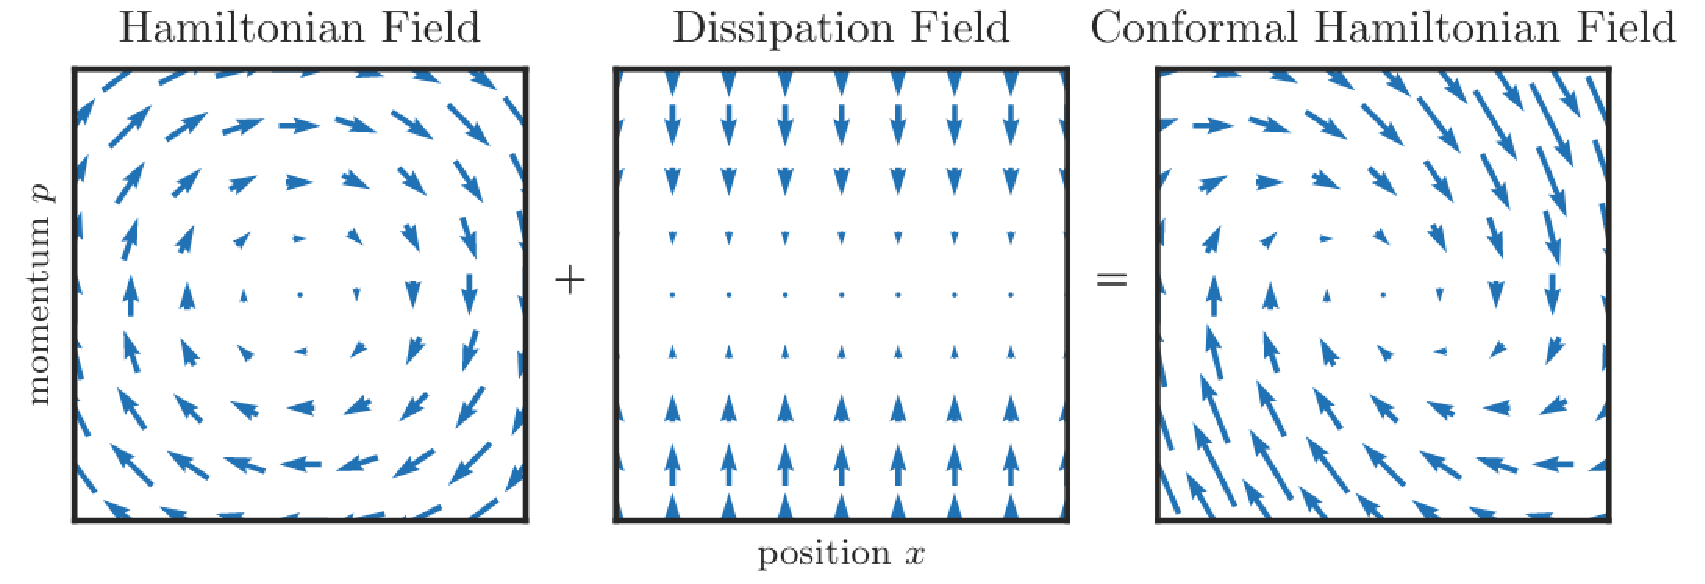
\includegraphics[width=\linewidth]{pics/conformal_hamiltonian.pdf}
%    \caption{Representation of the effect of a conformal Hamiltonian on the phase space in 1 dimension, from %\cite{maddison2018hamiltonian}.}
%    \label{fig:conf_hamiltonian}
%\end{figure}
These constraints naturally lead to use a  conformal Hamiltonian dynamics, as suggested in
\cite{rotskoff:vanden-eijden:2019}.  Assume that $U(\cdot) = \log \pi(\cdot)$ is continuously differentiable. We consider an extended distribution $\tilde\pi(q,p) \propto \exp \{-U(q)-K(p)\}$
on  $\rset^{2d}$, where $K:p\mapsto p^T\mass^{-1} p/2$, with $\mass$ a positive definite mass matrix. Note that $\pi$ is the marginal of $\tilde{\pi}$. In this setting, $q\in \rset^d$ is the position and $U(q)$ is the {\em potential energy}, while $p\in \rset^d$ is the momentum and $K(p)$ is the {\em kinetic energy}, by analogy with physics. The conformal Hamiltonian ODE associated with $\tilde \pi$ is defined by %(DHODE)
\begin{align}
  \label{eq:ODE_hamiltonian}
%\begin{aligned}
  &\rmd{q_t}/\rmd t =\nabla_{p} H(q_t,p_t) = \mass^{-1} p_t \eqsp, \\
  \nonumber
&\rmd {p}_t/\rmd t =-\nabla_{q} H(q_t,p_t)-\gamma p_t = -\nabla U(q_t) - \gamma p_t \eqsp,
\end{align}
where $H(q,p)= U(q)+ K(p)$, and $\gamma >0$ is a damping constant.
%the target
%$x = (p,q) \in \rset^{n}$ and $n=2d$. In practice, the prior $\rho$
%and the target $\pi$ are product of the form $\rho_q(q) \rho_p(p)$ and
%$\pi_q(q) \rho_p(p)$, where $\rho_q,\rho_p$ are density over $\rset^d$
%and $\pi_q(q) = \likelihood_q(q) \rho_q(q)/\const_q$, with $\const_q$ intractable.
% \subsection{Non-equilibrium Hamiltonian importance sampling estimators of $Z$ and $\pi$}\label{subsec:NISHamiltonianestimators}
%%The conformal Hamiltonian ODE is defined by %(DHODE)
%\begin{align}
%  \label{eq:ODE_hamiltonian}
%\begin{aligned}
%  &\dot{q}_t=\nabla_{p} H(q_t,p_t) =  p_t  \eqsp, \\
%  \nonumber
%&\dot{p}_t=-\nabla_{q} H(q_t,p_t)-\gamma p_t = -\nabla U(q_t) - \gamma
%p_t \eqsp,
%\end{align}
%where $H(q,p)=U(q)+ p^T p/2$, and $\gamma >0$ is a damping constant
%responsible for dissipating the energy of the system.
Any solution $(q_t,p_t)_{t \geq 0}$ of \eqref{eq:ODE_hamiltonian} satisfies $\rmd {H}/\rmd t (q_t,p_t) = - \gamma p_t^T\mass^{-1} p_t\leq 0$. Hence, all orbits converge to fixed points that satisfy $\nabla U(q)=0$ and $p=0$; see e.g. \citep{francca2019conformal,maddison2018hamiltonian}.
% We display in \Cref{fig:conf_hamiltonian} the phase plane of a conformal Hamiltonian dynamics system \eqref{eq:ODE_hamiltonian}. %\cite{rotskoff:vanden-eijden:2019} proposed to set $U(q) = -\log(\pi_q(q))$
%in the setting described above.
%Therefore, the transformation $\transfo$ can be seen as an optimization operator, which creates a path converging to the minimums of $U$,

%iteratively tries to find an optimum of the likelihood, see % Based on
% this result, \cite{rotskoff:vanden-eijden:2019} suggests to use
% \eqref{eq:ODE_hamiltonian} to apply their method.
%However, continuous
% dynamics cannot be used as such in practice: either the Hamiltonian ODE
% cannot be explicitly solved or it involves continuous integral which
% needs to be approximated.  To deal with this limitation,
 \begin{figure*}[h!]
     \centering
\begin{tabular}{cccc}
    % 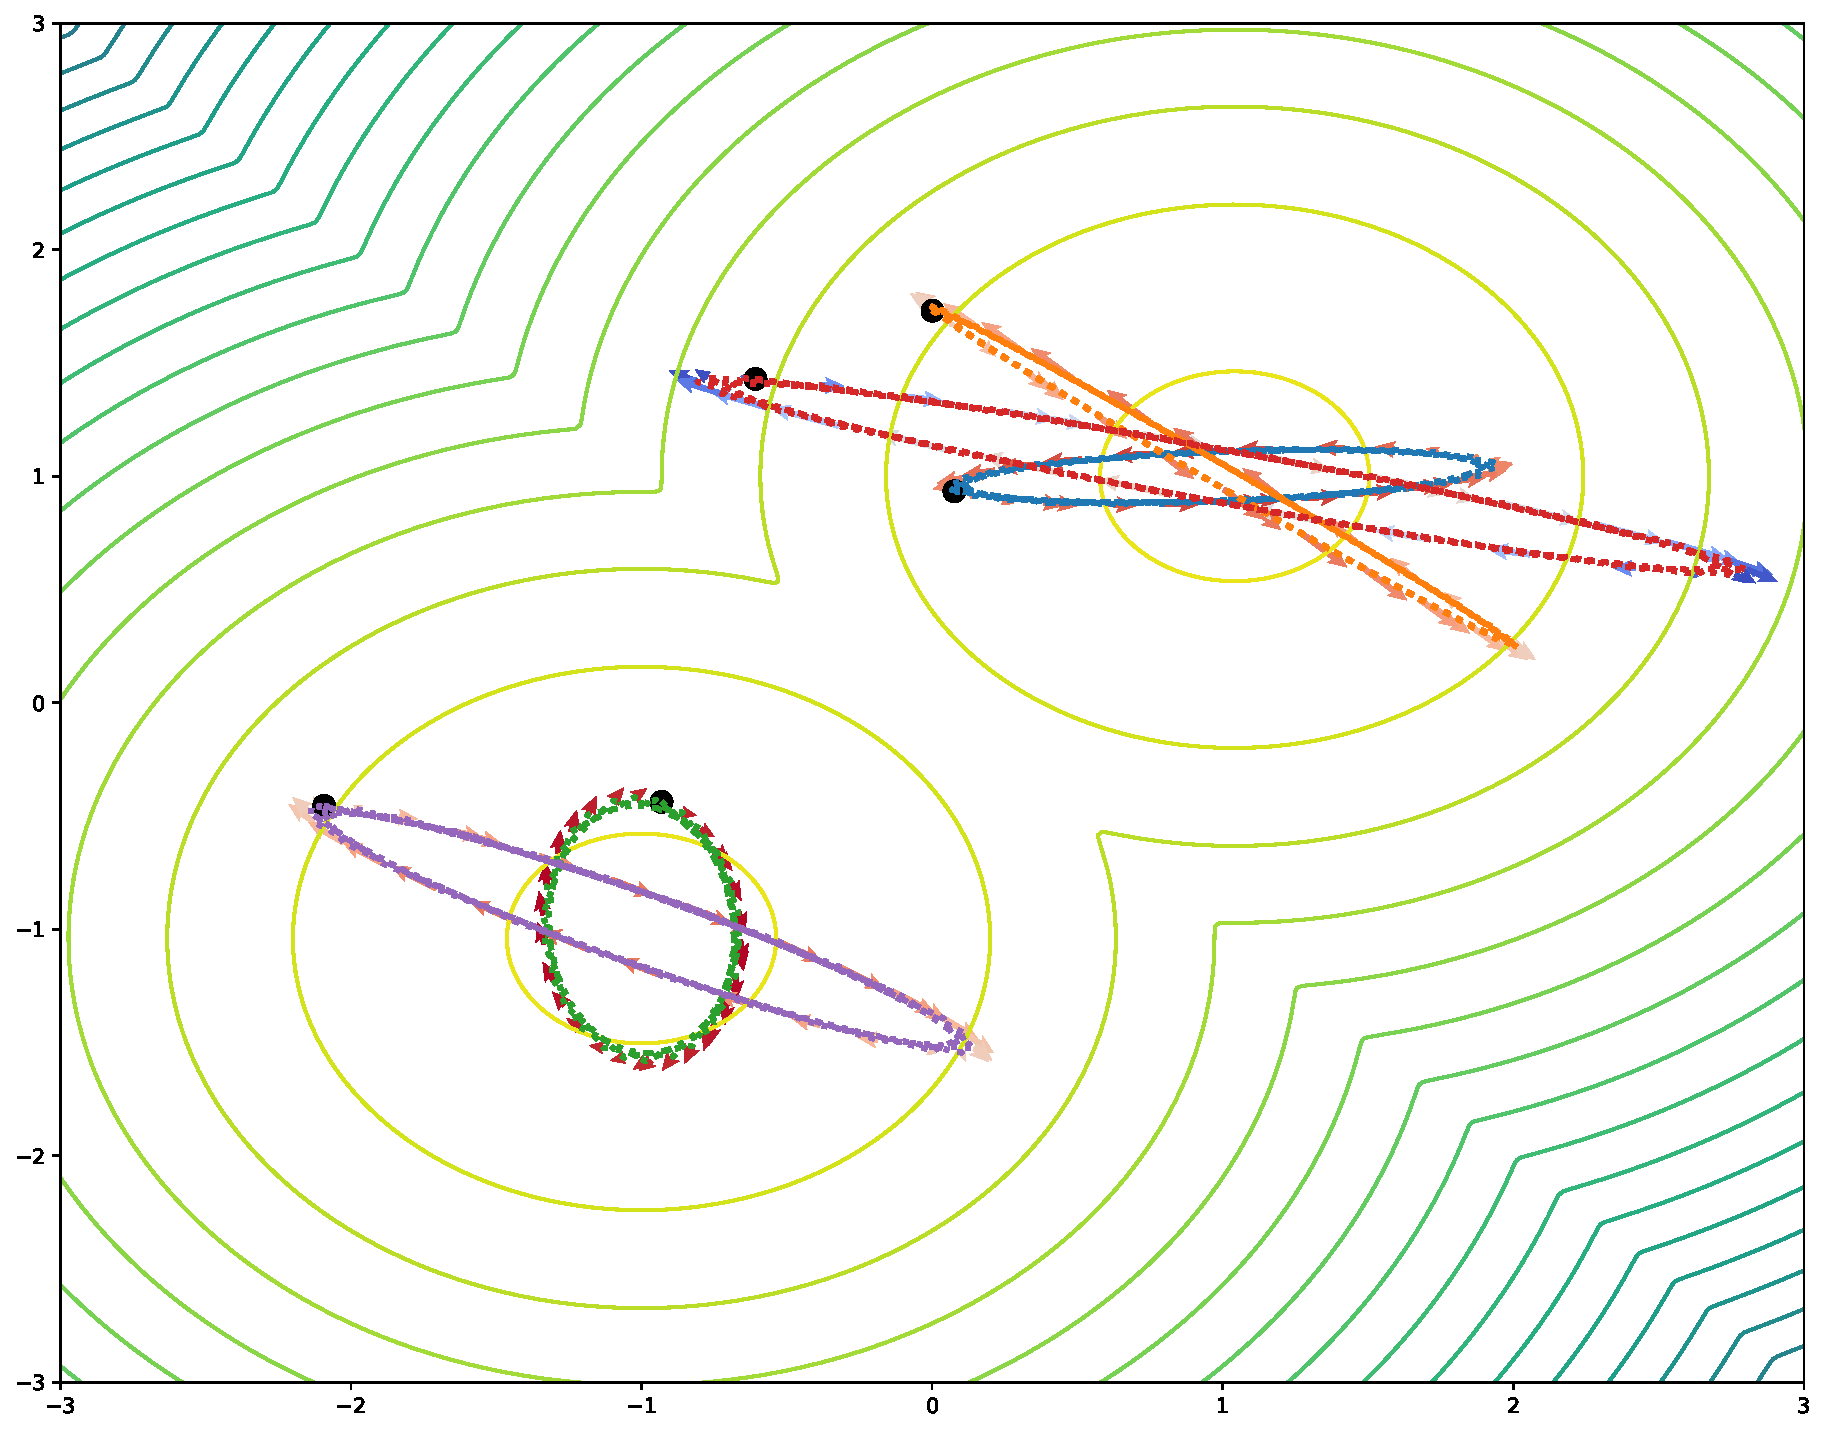
\includegraphics[width=0.25\linewidth]{pics/gamma0.0K30h0.1.pdf} & \includegraphics[width=0.25\linewidth]{pics/gamma0.3K30h0.1.pdf} & 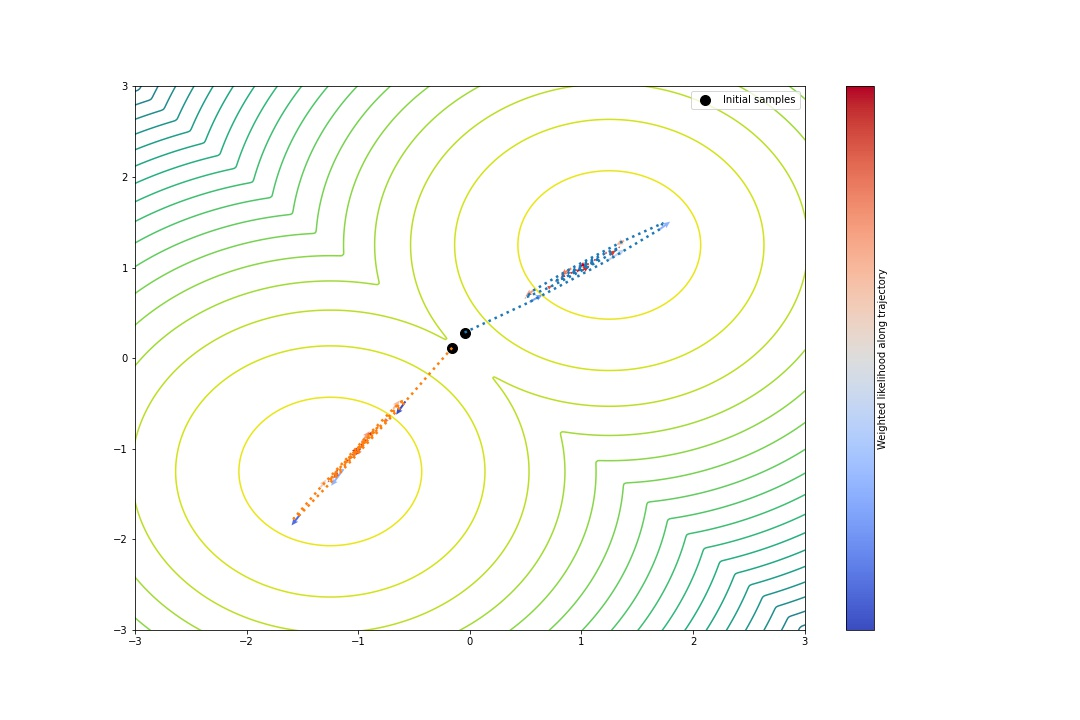
\includegraphics[width=0.25\linewidth]{pics/gamma2.0K30h0.1.pdf} &
     %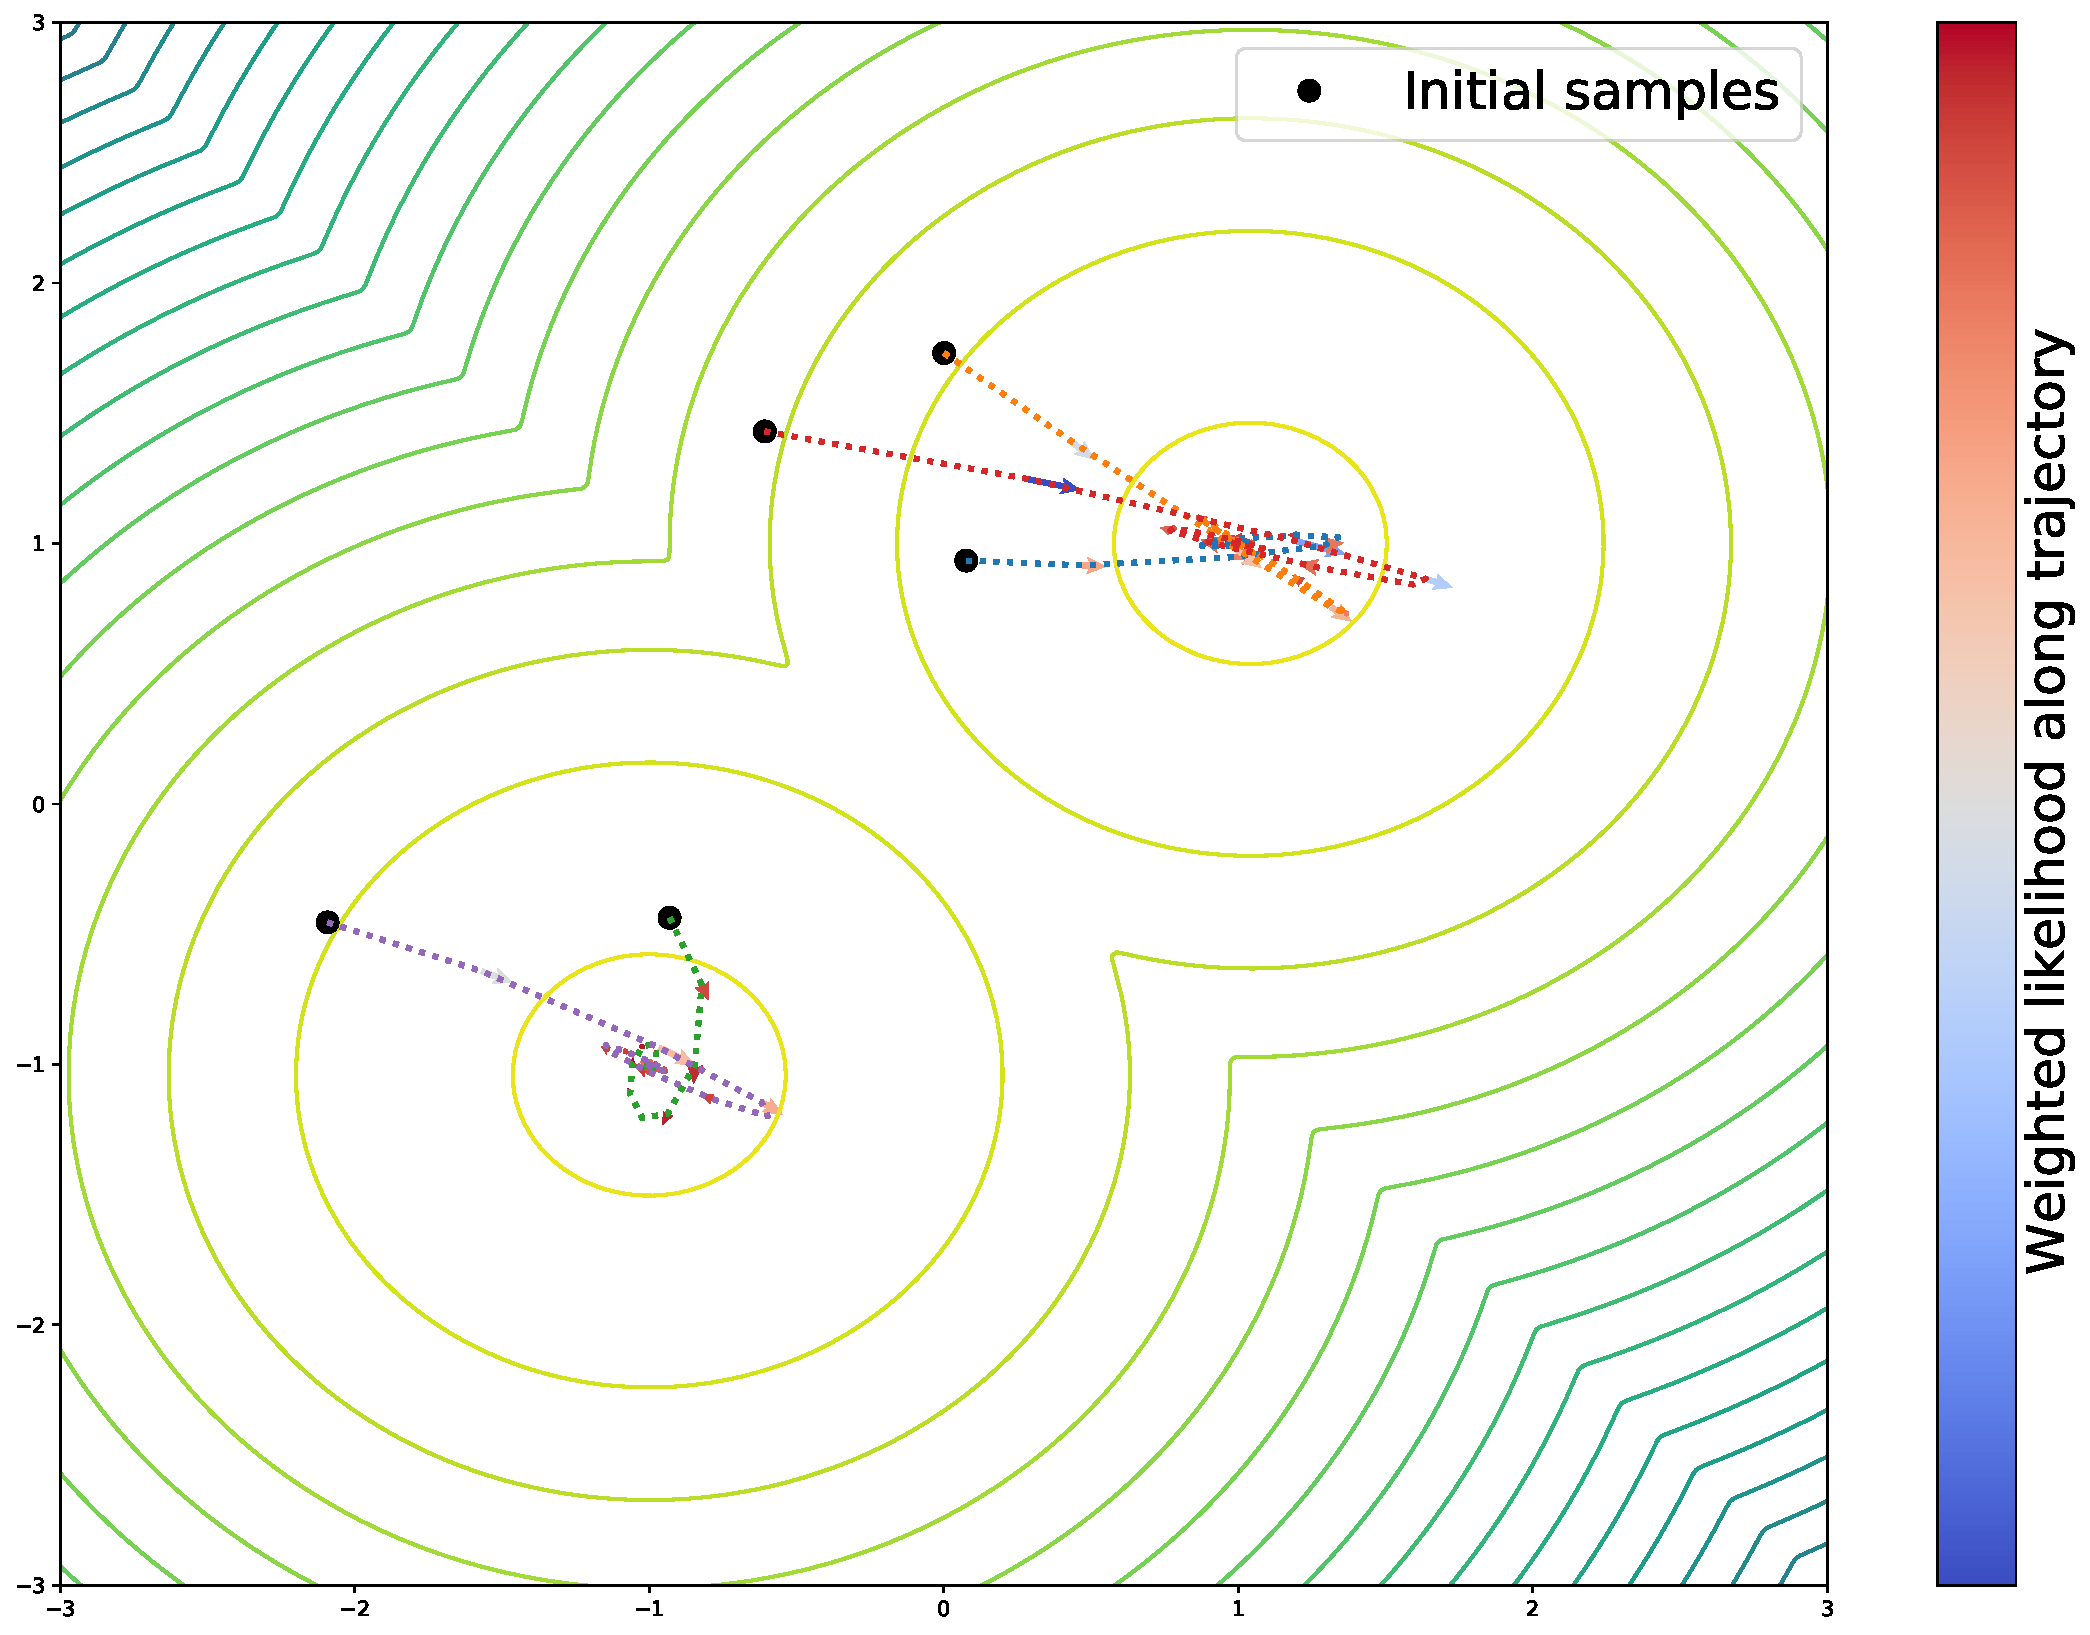
\includegraphics[width=0.25\linewidth]{pics/gamma5.0K30h0.1.pdf}
     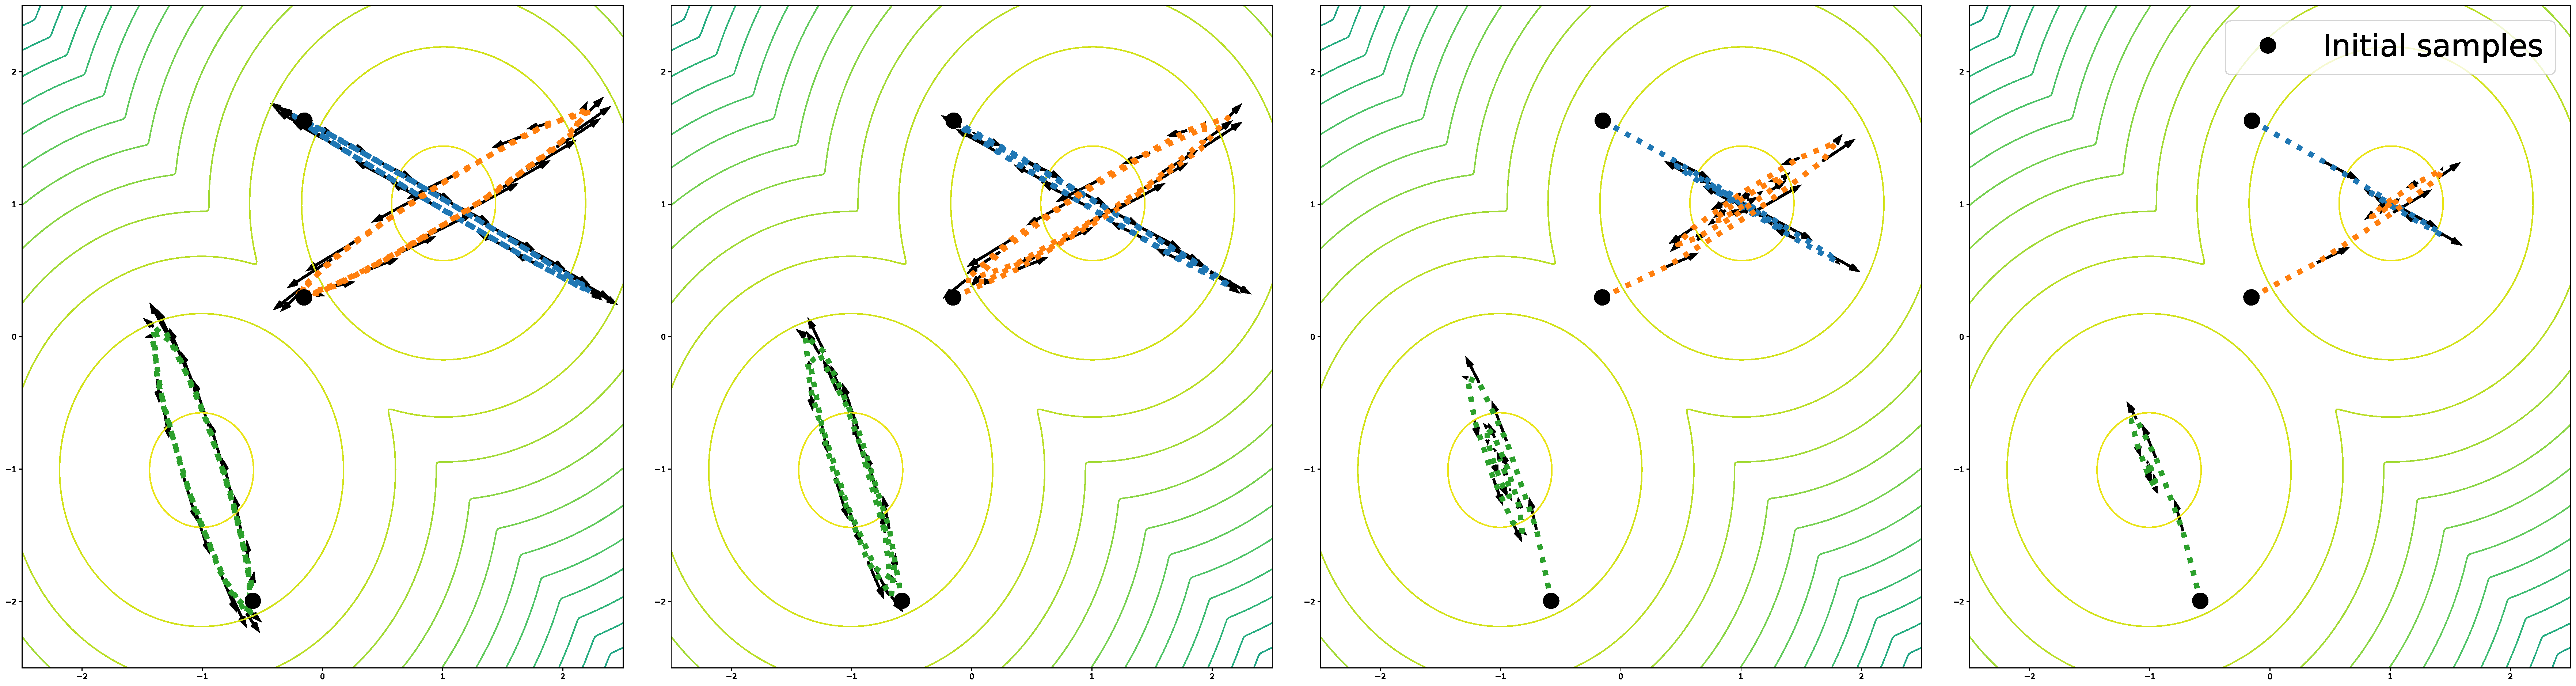
\includegraphics[width=1\linewidth]{pics/bigplot.pdf}
\end{tabular}
     \caption{Conformal Hamiltonian paths for different values of the dissipation parameters for a mixture of two Gaussian distributions given different Hamiltonian parameters. From left to right, $\gamma$ increasing from 0 to 0.3, 2 and 4.}
     \label{fig:toy_example_posterior}
 \end{figure*}
In the applications below, we consider the conformal version of the symplectic Euler method of \eqref{eq:ODE_hamiltonian}, see \cite{francca2019conformal}.
This integrator can be constructed as a splitting of the two conformal and conservative parts of the system \eqref{eq:ODE_hamiltonian}. When composing a dissipative with a  symplectic operator, we set for all $(q,p) \in \rset^{2dn}$, $\transfo_h(q,p)$ to be
%\begin{equation*}
 %\label{eq:def_psi_h}
 \[%\begin{multline*}
 %\transfo_h(q,p) =
 (q+h\mass^{-1}\{ \rme^{-h\gamma} p -h \nabla U(q)\},%\\  \quad
 \rme^{-h \gamma } p -h \nabla U(q))\eqsp,
\]%\end{multline*}
where $h >0$ is a discretization stepsize.
This transformation can be connected with classical momentum optimization schemes, see \citep[Section 4]{francca2019conformal}.
By \citep[Section 3]{francca2019conformal}, for any $h >0$ $\transfo_h$ is a $\rmC^1$-diffeomorphism on $\rset^{2d}$ with Jacobian given by $\JacOp{\transfo_h}(q,p) = \rme^{-\gamma h d}$. In addition,  its inverse is
$  \transfo_h^{
-1}(q,p) = (q-h\mass^{-1} p,\rme^{\gamma h}\{p+h \nabla U(q-h\mass^{-1} p)\})$.
% \begin{equation}
%   \label{eq:def_phi_h_inverse}
%  \eqsp.
% \end{equation}
Therefore, the weight \eqref{eq:def_w_k} of the  \IFIS\  estimator is given by
\begin{equation}
w_{k}(q,p) = \frac{ \tilde \rho(\transfo^k_h(q,p)) \rme^{-\gamma k h d} }{
    \sum_{j = k-K}^k  \tilde \rho(\transfo^j_h(q,p)) \rme^{-\gamma j h d} },
\end{equation}
where $\tilde \rho(q,p) \propto \rho(q) \rme^{-K(p)}$.
In the applications below, $\mass$ is chosen as a diagonal matrix with positive entries, see the  discussion  in \Cref{subsec:estim_constant}.

\section{InFiNE-based MCMC}\label{sec:infine:MCMC}
We describe here novel MCMC algorithms that leverage the $\InFiNE$ method to sample from $\pi$.

To motivate our sampler, let us recall the principle of the Sampling Importance Resampling method (SIR; \citet{rubin1987comment,smith1992bayesian}) whose goal is to approximately sample from the target distribution $\target$ using samples drawn from a proposal distribution $\proposal$.

In SIR, a $N$-\iid\ sample $\chunku{X}{1}{N}$ is first generated from the proposal distribution $\proposal$. A sample $X^*$ is approximately drawn from the target $\target$ by choosing randomly a value in $\chunku{X}{1}{N}$ with probabilities proportional to the importance weights $\{\weightfunc(X^i)\}_{i = 1}^N$, where $\weightfunc(x)= \target(x)/\proposal(x)$. Note that the importance weights are required to be known only up to a constant factor.  For SIR, as $N \to \infty$, the sample $X^*$ is \emph{asymptotically} distributed according to $\target$; see~\cite{smith1992bayesian}. Two major drawbacks of SIR are that it is only asymptotically valid and that the number $N$ of proposals should typically grow exponentially with the dimension $d$ of the state-space to maintain a given accuracy.

A subsequent algorithm  is the \emph{iterated SIR} (ISIR) \citep{andrieu2010particle}. In this version, the sample size $N$ is not necessarily large ($N\geq 2$), but the whole process of sampling a set of proposals, computing the importance weights, and picking a  candidate, is iterated. At the $n$-th step of ISIR, the
%\xian{I would switch to passive and remove all the we}
active set of $N$ proposals $\chunku{X_n}{1}{N}$ and the index $I_n \in [N]$ of the conditioning proposal are kept. First ISIR  updates the active set  by setting $X_{n+1}^{I_n}= X_n^{I_n}$ (keep the conditioning proposal) and then draw independently $\chunkum{X_{n+1}}{1}{N}{I_n}$ from $\proposal$.
Then it selects the next proposal index $I_{n+1} \in [N]$ by sampling with probability
proportional to $\{\weightfunc(X_{n+1}^i)\}_{i=1}^N$.
As shown in \cite{andrieu2010particle}, this algorithm  defines  a partially collapsed Gibbs sampler (PCG) of the augmented distribution (see \Cref{subsec:ISIR-partially-collapsed-dependent})
$$%\begin{equation*}
\bar{\measpi}(\chunku{x}{1}{N},i)=\frac{1}{N}  \target(x^i) \prod_{j \neq i} \proposal(x^j) =\frac{1}{N} \weightfunc(x^i) \prod_{j=1}^N \proposal(x^j) \eqsp.
$$%\end{equation*}
The PCG sampler can be shown to be ergodic provided that $\proposal$ and $\target$ are continuous and $\proposal$  is  positive on the support of $\target$. If in addition the importance weights are bounded, the Gibbs sampler can be shown to be uniformly geometrically ergodic  \citep{lindsten2015uniform,andrieu2018uniform}.
It follows that the distribution of the conditioning proposal $X_n^*= X_n^{I_n}$ converges to $\pi$ as the iteration index $n$ goes to infinity. Indeed, for any integrable function $f$ on $\rset^d$, with $(\chunk{X}{1}{N},I) \sim \bar{\measpi}$,
\begin{multline*}
\allowdisplaybreaks
\PE_{}[f(X^I)]= \int \sum_{i=1}^N f(x^i)  \bar{\measpi}(\chunku{x}{1}{N},i) \rmd \chunku{x}{1}{N} \\
\allowdisplaybreaks
= N^{-1} \sum_{i=1}^N \int f(x^i) \target(x^i) \rmd x_i = \int f(x) \target(x) \rmd x \eqsp.
\end{multline*}
When the state space dimension $d$ increases, designing a proposal distribution $\proposal$ guaranteeing proper mixing properties becomes more and more difficult. A way to circumvent this problem is to use dependent proposals, allowing in particular \emph{local moves} around the conditioning path. To implement this idea, for each $i \in [N]$, we define a proposal transition, $r_i(x^i; \chunkum{x}{1}{N}{i})$ which defines the the conditional distribution of $\chunkum{X}{1}{N}{i}$ given  $X^i= x^i$. The key property validating ISIR with dependent proposals (see \Cref{subsec:ISIR-partially-collapsed-dependent}) is that all one-dimensional marginal distributions are equal to $\proposal$, which requires that for each $i,j  \in [N]$,
\begin{equation}
\label{eq:conditional-decomposition}
\proposal(x^i) r_i(x^i;\chunkum{x}{1}{N}{i})=
\proposal(x^j) r_j(x^{j};\chunkum{x}{1}{N}{j})
\end{equation}
The (unconditional) joint distribution of the particles is therefore defined as
\begin{equation}
\label{eq:joint-distribution}
\proposal_N\bigl(\chunku{x}{1}{N}\bigr) = \proposal(x^1) r_1(x^1;\chunkum{x}{1}{N}{1}) \eqsp.
\end{equation}
The resulting modification of the ISIR algorithm is straightforward: $\chunkum{X}{1}{N}{I_n}$ is sampled jointly from the conditional distribution $r_{I_n}(X_n^{I_n},\cdot)$ rather than independently from $\proposal$.

There are many ways to make proposals dependent. For instance, dependence may be induced by using a Markov kernel reversible \wrt\ to the proposal $\proposal$, i.e., such that $\proposal(x) m(x,x')= \proposal(x') m(x',x)$, assuming for simplicity that this kernel has density $m(x,x')$ \citep{ruiz:titsias:doucet:2020}. In this case, for each $i \in [N]$, the conditional proposal kernel is
\begin{multline}
\label{eq:condition-kernel}
r_i(x^i,\chunkum{x}{1}{N}{i}) \\ =
\prod_{j=1}^{i-1} m(x^{j+1},x^{j}) \prod_{j=i+1}^n m(x^{j-1},x^j) \eqsp.
\end{multline}
A straightforward induction shows that \eqref{eq:conditional-decomposition} is satisfied and that the joint distribution of the particles (see \eqref{eq:joint-distribution} is given by  $\proposal_N(\chunku{x}{1}{N})=\proposal(x^i) \prod_{j=2}^{N} m(x^{j-1},x^j)$. If $\proposal$ is Gaussian, an appropriate choice is an autoregressive kernel $m(x,x')= \phi_d(x';\alpha x, \sqrt{1-\alpha^2} \Id_d)$, where $\phi_d(x; \mu, \Sigma)$ is the $d$-dimensional Gaussian pdf with mean $\mu$ and covariance $\Sigma$ as in  \citep{ruiz:titsias:doucet:2020}. More generally, we can use a Metropolis-Hastings kernel with invariant distribution $\proposal$.

 We now propose the \IFIS\ MCMC sampler which extends the ISIR algorithm to \IFIS\ construction.  The input for the $n$-th iteration comprises an active set  of $N$ path initial states,  $\chunku{X}{1}{N}$, the index $1\le I_n\le N$ of the conditioning path, and the iteration index $0\le K_n\le K$ along the conditioning path. %As summarized in \Cref{algo:IFIS-MCMC}, the
Adopting the ISIR protocol, our sampler proceeds as follows.
\begin{enumerate}
\item Set  $X_{n+1}^{I_n}= X_n^{I_n}$ and draw the remaining proposals $\chunkum{X_{n+1}}{1}{N}{I_{n}} \sim r_{I_n}(X^{I_n},\cdot)$.
\item For each initial value $X_{n+1}^i$, $i \in [N]$, compute the iterates $\{ \transfo^k(X_{n+1}^i) \}_{k=1}^K$.
\item Draw the path index $I_{n+1}  \in [N]$  with probability proportional to  $(\estConstC{X_{n+1}^{i}})_{i \in [N]}$, with $\estConstC{X_{n+1}^{i}}$ defined in  \eqref{eq:def_estimator_normal_const_1}.
\item Draw the next iteration  index $0\le K_{n+1} \le K$ on the conditioning path with probability proportional to
\[
%\omega_{k,n+1}=
\w_k(X^{I_{n+1}}_{n+1})\likelihood(\transfo^k(X^{I_{n+1}}_{n+1})) \eqsp.
\]
\end{enumerate}
%\begin{algorithm}[t]
%\caption{\IFIS\ MCMC}
%\begin{enumerate}[wide, labelwidth=!, labelindent=0pt, %label=(\arabic*)]
%\item Set $X_{n+1}^{I_{n}}= X_n^{I_n}$ and draw %$\chunkum{X_{n+1}}{1}{N}{I_n} \sim r_{I_n}(X_n^{I_n},\cdot)$
%\item For $i \in [N]$, compute $\{\transfo^k(X_{n+1}^i)\}_{k=0}^K$
%\item Draw $I_{n+1} \sim %\operatorname{Cat}[(\estConstC{X_{n+1}^{i}})_{i \in [N]}]$
%\item Draw $K_{n+1} \sim %\operatorname{Cat}[(\omega_{k,n+1})_{k=0}^K]$
%\end{enumerate}
%\label{algo:IFIS-MCMC}
%\end{algorithm}
Similar to ISIR, \IFIS\ MCMC is a partially collapsed Gibbs sampler targeting the extended pdf (see \Cref{subsec:partial-collapsed-infine}) %textcolor{red}{this way of defining the target is not very informative, it is simply $\bar{\measpi}(\chunku{x}{1}{N},i)=\frac{1}{N}  \target(x^i) r_{i}(x^i,\chunkum{x}{1}{N}{i})$ from which it is trivial again that marginal $X^I \sim \pi$ so we don't need to detail the calculations}
%% eric: on fait apparaitre $k$ dans la loi jointe pour bien faire comprendre que l'on tire d'abord $I$ puis $K$. C'est exactement la loi dont on a besoi dans la suite
\begin{align}\label{eq:def_measpi_N}
\nonumber
&  \bar{\measpi}(x^{1:N},i,k) \\
\nonumber
  &= {\w_k(x^i)\likelihood(\transfo^{k}(x^i) \proposal(x^i) r_i(x^i;\chunkum{x}{1}{N}{i})}\big/{N \const} \\
  &= {\w_k(x^i)\likelihood(\transfo^{k}(x^i)
  )}\proposal_N(\chunku{x}{1}{N})\big/{N \const}
   \eqsp.
\end{align}
whose marginal distribution satisfies
\[
\bar{\measpi}(\chunku{x}{1}{N},i)=\frac{1}{N \const}  \estConstC{x^i} \proposal(x^i) r_i(x^i;\chunkum{x}{1}{N}{i})\eqsp.
\]
Under mild conditions (see \Cref{sup:sec:ergodicity}), this PCG sampler is ergodic, hence the distributions of the iterates $(\chunku{X_n}{1}{N},I_n,K_n)$ and of their projections $X^*_n=\transfo^{K_{n}}(X_n^{I_n})$ converge to $\bar{\measpi}$ and to $\target$, respectively. Indeed, for any integrable function $f$ on $\rset^d$, with $(\chunk{X}{1}{N},I,K)\sim \bar{\measpi}$,
 \begin{align*}
    & \PE[f(T^K(X^I))]= \sum_{i=1}^N\int_{}\sum_{k=0}^K\bar{\measpi}(x^{1:N},i,k)f(T^k(x^i))
    \rmd \chunku{x}{1}{N}  \\
    &=(N \const)^{-1}\! \sum_{i=1}^N\!\int_{}\sum_{k=0}^K   \rho(x^i) \w_k(x^i)  \likelihood(\transfo^{k}(x^i))f(\transfo^k(x^i)) \rmd x^i
    \\
    & = (N \const)^{-1} \sum_{i=1}^N\int_{} \rho(x^i) \likelihood(x^i)f(x^i) \rmd x^i = \int_{} \measpi(y)f(y) \rmd y \eqsp,
\end{align*}
following \Cref{theo:inf_non_eq}.
%\end{proof}
The \IFIS\  MCMC sampler is thus a valid procedure to generate samples from $\measpi$. When the transformation $\transfo$ is chosen as in \Cref{subsec:NISestimators}, our sampler draws samples based on optimization paths. Detailed experiments are discussed in \Cref{subsec:mcmc_exp}.

% $ \breve{\measpi}(\rmd y)=\sum_{k \in \zset} \int \breve{\measpi}( \rmd x, k, \rmd y)=\measpi(\rmd y)$.
%for $\estConstC{x^{1:N}}$ defined in \eqref{eq:def_estimator_normal_const}. Similarly, we show that IFG described in \Cref{algo:gibbs_partial} is a partially collapsed Gibbs sampler targeting \eqref{eq:def_measpi_N}.


% Regarding the Indeed, sampling $\tilde{Y}$ from this distribution is equivalent to Step 1-Step 2 of \Cref{algo:IMH} and we can additionally check that the Radon-Nikodym derivative between these two distributions satisfies\arnaud{maybe this should be detailed as this is really key}
% where $p_k^i$ is defined in \eqref{eq:def_estimator_naive_monte_carlo}. The acceptance probability in Step 3 of  \Cref{algo:IMH}  follows directly.

%****We need to add the proof of validity of the Gibbs algorithm here***

%It can similarly checked that the `local' partially collapsed Gibbs sampler targets the modified extended target
%\begin{align}
%  \label{eq:def_measpi_N_gibbs}
%  \bar{\measpi} (\rmd x^{1:N},i,k,\rmd y)  &=  N^{-1} \breve{\measpi}(\rmd x^i,k,\rmd y)  \textstyle{\{\prod_{j= i}^{N} M(x^j,\rmd x^{j+1})\}\{\prod_{j= 1}^{i-1} M(x^{j+1},\rmd x^{j})\}} \eqsp,
%\end{align}
%which also satisfies $  \bar{\measpi} (\rmd y)= \pi(\rmd y)$ by \Cref{corollary:inv_kernel} and \eqref{eq:kernel}.

% is now modified, as $\bar{\measpi}^N(\rmd x^{1:N}| (i,k,y)) = \updelta_{\transfo^{-k}(y)}(\rmd
% x^i)\textstyle{\{\prod_{j= i}^{N-1} M(x^j,\rmd x^{j+1})\}M(x^N, \rmd x^1)\{\prod_{j= 1}^{i-2} M(x^j,\rmd x^{j+1})\}}$. Sampling $X^{1:N} $ The rest stays untouched. By picking $M$ appropriately, we propose new particles close to the ``active'' particle $X^I$.
% Note here that a sensible algorithm would balance out contribution from a kernel $M$ to propose local moves from the active particle and the prior $\rho$ to ensure that we explore all possible modes of the posterior distribution $\pi$.


\section{ELBO for variational auto-encoders}
\label{sec:extensions}
%The performance of the $\IFIS$ estimators depend crucially on the non-equilibrium transformations. Consider here a family of invertible flows $\{ \transfo_{k,\psi} \, : \, \psi \in \rset^{p}\}_{k\in\nsets}$ and estimate $\psi$ optimizing a variational criterion. For simplicity of notation, for the moment, we will omit parameters $\psi$ in the following.
%Moreover, notice that the unbiased estimation of a normalizing constant we provide is all that is required to define an ELBO for learning generative models, such as a VAE \cite{kingma:welling:2013}.
\begin{comment}
For high dimensional observations $y$, Variational Auto-Encoders (VAE)  build upon some latent variables $x\in\rset^d$ to define a likelihood model as
\begin{equation}\label{eq:demarge}
p_\theta(y) = \int p_\theta(y\mid x) p(x) \rmd x = \int p_\theta(x,y) \rmd x\eqsp.
\end{equation}
As this integral representation is not tractable, and approximating it naively by Monte Carlo would result in a large variance, \cite{kingma:welling:2013} introduced a parametric family of distributions $\{q_\phi(\cdot\mid y)\}_\phi$ approximating $p_\theta(\cdot\mid y)$.
\end{comment}
Given a joint model $p_\theta(y, x)$, with data $y \in \rset^p$ and latent variable $x \in \rset^d$, variational inference (VI)
provides us with a tool to both approximate the intractable
posterior $p_\theta(x|y)$ and maximize the marginal likelihood
$p_\theta(y)= \int p_\theta(x,y) \rmd x$ in the parameter $\theta$. This is achieved by introducing a
parameterized approximate posterior $q_\phi(x|y)$ and maximizing
the Evidence Lower Bound (ELBO) (see \cite{kingma2019introduction})
\begin{align}\label{eq:elbo}
\mathcal{L}_{\textup{ELBO}}(\theta,\phi)&= \int \log\left(\frac{p_\theta(x,y)}{q_\phi(x\mid y)}\right) q_\phi(x\mid y)\rmd x \eqsp\\
&=\log p_\theta(y)-\operatorname{KL}(q_\phi(\cdot\mid y) \| p_\theta(\cdot\mid y) )\eqsp,\nonumber
\end{align}
where $\operatorname{KL}$ is the Kullback–Leibler divergence.
Towards more flexibility, approximate posteriors can be defined as marginal distributions, $q_\phi(x|y) = \int
\bar{q}_\phi (x, u |y) \rmd u$, where $u \in \mathsf{U}$ is an auxiliary variable (which can both have discrete ann dontinuous components) and $\bar{q}_\phi(x,u|y)$ is a generative closed-form density. %auxiliary variational inference (AVI).
Introducing auxiliary variables loses the tractability of \eqref{eq:elbo} but they allow for their own ELBO as suggested in \cite{agakov2004auxiliary}; \cite{lawson2019energy}, leading to the objective
\begin{equation}\label{eq:AVI_ELBO}
\int \bar{q}_\phi(x,u|y) \log \left( \frac{\bar{p}_\theta(x,u,y)}{\bar{q}_\phi(x,u|y)} \right)  \rmd x \rmd u \eqsp,
\end{equation}
where $\bar{p}_\theta(x,u,y)$ is an extended joint likelihood satisfying $p_\theta(x,y)= \int \bar{p}_\theta(x,u,y) \rmd u$ (or equivalently $\bar{p}_\theta(x,u,y)= p_\theta(x,y) \bar{m}_\theta(x,y; u)$ where $\bar{m}_\theta(x,y;\cdot)$ is a Markov kernel).
We now exploit this idea within the \IFIS\ framework. For that purpose, set prior, likelihood, and posterior as $\proposal(x)=q_\phi(x\mid y)$, $\likelihood(x)= p_\theta(x,y)/ q_\phi(x \mid y)$, and $\target(x)=p_{\theta}(x\mid y)$, respectively (the dependence of $\proposal$, $\likelihood$, and $\target$ on both parameter $(\theta$, $\phi)$ and observation $y$ is implicit for notational simplicity). With these notations, the normalizing constant of $\proposal(x) \likelihood(x)$ is then  $\const= p_\theta(y)$. The auxiliary variable $u$ is naturally associated with the extended target $\bar{\measpi}$ defined in \eqref{eq:def_measpi_N} (playing the role of $\bar{p}_\theta$), with
$$(x,u)=([x,\chunkum{x}{1}{N}{i}],i,k)$$
%$$(x,u)=(\chunku{x}{1}{N},i,k)$$
$[x,\chunkum{x}{1}{N}{i}]$ being a shorthand notation for a $N$-tuple $\chunku{x}{1}{N}$ with $x^i= x$. An extended proposal playing the role of $ \bar{q}_\phi(x,u|y)$ is derived from the \IFIS~MCMC sampler, i.e.
\begin{equation}
\label{eq:proposal-extended}
\bar{\proposal}(\chunku{x}{1}{N},i,k)=  \frac{\likelihood(\transfo^k(x^i)) \w_k(x^i)}{N \estConstC{\chunku{x}{1}{N}}} \proposal_N(\chunk{x}{1}{N})  \eqsp.
\end{equation}
where $\estConstC{\chunku{x}{1}{N}}$ is the \IFIS\ estimator \eqref{eq:def_estimator_normal_const} of the normalizing constant.
Note that, by construction, 
\begin{equation}
\label{eq:expression-marginal}
\sum_{i=1}^N \sum_{k=0}^K \bar{\proposal}(\chunku{x}{1}{N},i,k) = \proposal_N(\chunku{x}{1}{N})
\end{equation}
showing that this joint proposal can be sampled by drawing the proposals $\chunku{x}{1}{N} \sim \rho_N$, then sampling the path index $i \in [N]$ with probability proportional to $(\estConstC{x^i})_{i=1}^N$ (with $\estConstC{x}$ defined in \eqref{eq:def_estimator_normal_const_1}) and finally the iteration index $k \in \{0,\dots,K\}$ with probability proportional to $(\w_k(x^{i})\likelihood(\transfo^k(x^{i}))_{k=0}^K$.
\begin{comment}
this lower bound can be inaccurate. To improve it, we can exploit any unbiased positive estimate $\hat{p}_{\theta}(y)$ of the marginal likelihood.
%with variance lower than the ratio  $p_\theta(x,y)/q_\phi(x\mid y),~x\sim q_\phi(\cdot | y)$, exploited in \cref{eq:elbo} to define a valid ELBO \cite{mnih2016variational}.
Indeed $\log p_\theta(y)= \log \mathbb{E}[\hat{p}_{\theta}(y)]\geq \mathbb{E}[\log \hat{p}_{\theta}(y)]$ by Jensen's inequality.
\cite{mnih2016variational} argue that the better the estimator $\hat{p}_\theta(y)$, the better the ELBO.
\end{comment}
Since the ratio of \eqref{eq:def_measpi_N} over \eqref{eq:proposal-extended} is
\begin{equation}
\label{eq:ratio-extended}
{\bar{\measpi}(\chunku{x}{1}{N},i,k)}\big/{\bar{\proposal}(\chunku{x}{1}{N},i,k)}= {\estConstC{\chunku{x}{1}{N}}}\big/{\const} \eqsp.
\end{equation}
The augmented ELBO   \eqref{eq:AVI_ELBO} writes
\begin{align}
 \label{eq:infine_elbo-alt}
\elboneq &= \int_{} \proposal_N( \chunku{x}{1}{N})   \log \estConstC{\chunku{x}{1}{N}} \rmd \chunku{x}{1}{N}\eqsp,\\
\nonumber
 &=  \log \const - \operatorname{KL}( \bar{\proposal} | \bar{\measpi} )\eqsp,
\end{align}
where we have used \eqref{eq:expression-marginal} and that the ratio ${\bar{\measpi}(\chunku{x}{1}{N},i,k)}\big/{\bar{\proposal}(\chunku{x}{1}{N},i,k)}$ does not depend on 
the path index $i$ and the proposal index $k$ along the path. When $K=0$ and $\proposal_N(\chunku{x}{1}{N})= \prod{j=1}^N \proposal(x^j)$, we exactly retrieve the Importance Weighted AutoEncoder (IWAE); see e.g.  \cite{burda:grosse:2015} and in particular the interpretation in \cite{cremer2017reinterpreting}. 

Choosing the conformal Hamiltonian introduced in \Cref{subsec:NISestimators} allows for a family of invertible flows that depends on the parameter $\theta$ which itself is directly linked to the target distribution.




%\begin{tabular}{ *2c }    \toprule
%\emph{10 ep., $d=64$, $K\in\{3,5,8\}$} & \emph{MNIST}  \\\midrule
%VAE    &  97.50  \\
%IWAE - $M=5$ & 96.98\\
%IWAE - $M=30$ & 96.97  \\
%NeqVAE - $\gamma = 0.1$, $h=0.1$ & $97.23\|97.22\|98.31$  \\
%NeqVAE - $\gamma = 0.3$, $h=0.1$ &  $97.25\|97.08\|101.99$\\
%NeqVAE - $\gamma = 0.5$, $h=0.1$ & $96.90\|97.42\| \mathrm{Na}$ \\
%NeqVAE - $\gamma = 0.1$, $h=0.05$ & $97.20\|97.02\|97.00$ \\
%NeqVAE - $\gamma = 0.1$, $h=0.01$ & $95.79\|95.77\|97.37$ \\
%NeqVAE - $\gamma = 0.3$, $h=0.01$ & $97.58\|97.28\|97.18$ \\
%NeqVAE - $\gamma = 0.5$, $h=0.01$ & $97.58\|97.69\|97.03$ \\
%\bottomrule
% \hline
%\end{tabular}

%\begin{tabular}{ *2c }    \toprule
%\emph{10 ep., $d=64$, $K\in\{3,5,8\}$} & %\emph{FashionMNIST}  \\\midrule
%VAE    &  238.90  \\
%IWAE - $M=5$ & 238.68\\
%IWAE - $M=30$ &  239.28 \\
%NeqVAE - $\gamma = 0.1$, $h=0.01$ & $239.87\|239.17\|239.45$ \\
%NeqVAE - $\gamma = 0.3$, $h=0.01$ & $239.70\|239.60\|239.53$ \\
%NeqVAE - $\gamma = 0.5$, $h=0.01$ & $239.37\|239.75\|239.39$ \\
%\bottomrule
% \hline
%\end{tabular}


\section{Numerical Experiments}
\subsection{Normalizing constant estimation}
\label{subsec:estim_constant}
We first consider the problem of the estimation of the normalizing constant of Gaussian mixtures in dimension $d$ in two different settings. In the first experiment, we consider an (unnormalized)  mixture of two Gaussian distributions, with equal mixing weights. The mean of the two components are set to $(\mathbf{1}_d, -\mathbf{1}_d)$, where $\mathbf{1}= [1,\dots,1]^T$ and covariance $\sigma ^2 \Id = 0.02$.
The second target is an unnormalized mixture of 25 $d$-dimensional Gaussian distributions in dimension $d=10,20$. Each component has the same covariance assumed to be diagonal with diagonal elements equal to $(0.01,0.01, 0.1, \ldots, 0.1)$. The means are given by $(i,j,0,\ldots,0)$ with $i,j \in \{-2,\ldots, 2\}$, see \Cref{fig:25_gauss_mcmc}.  The normalizing constant in this case is 12.5. In both examples the proposal $\rho$ is chosen to be a $d$-dimensional Gaussian, with zero mean and diagonal covariance $\sigma^2_\proposal \Id_d$, with $\sigma^2_\rho=5$. %We choose $d=10$ in our experiments. %Consider a flat proposal distribution $\rho$, which is assumed to cover the different modes of the target distribution.
The performance of the $\IFIS$ estimator \eqref{eq:def_estimator_normal_const} is first illustrated in this toy problem for $d\in\{5,10,15,20\}$ and different choices of parameters.

Our approach is compared with a na{\"\i}ve IS estimator using the same proposal $\rho$. %, which is assumed to cover the different modes of the target distribution.%, and would compute the estimator $\hat{Z}_n = 1/n \sum_{k\leq n} p(X^i)/\rho(X^i)$, where $x^i\sim \rho$.
A state-of-the-art competitor for the estimation of normalizing constants, the AIS estimator of \cite{neal:2001,tokdar2010importance} is also included in the comparison.
AIS relies on a sequence of target distribution $\target_k(x)$, $0 \leq k \leq K$ with $\target_0(x)= \proposal(x)$ and $\target_K(x)= \target(x)$. AIS defines an extended target and proposal using MCMC kernels which are reversible for each linking densities $\target_k$; most often, these MCMC kernels use Langevin or Hamiltonian dynamics; see \eg\ \cite{buchholz2021adaptive}. Therefore, AIS is directly comparable to the \IFIS\ estimator in terms of complexity.
\begin{figure}[!ht]
    \centering
    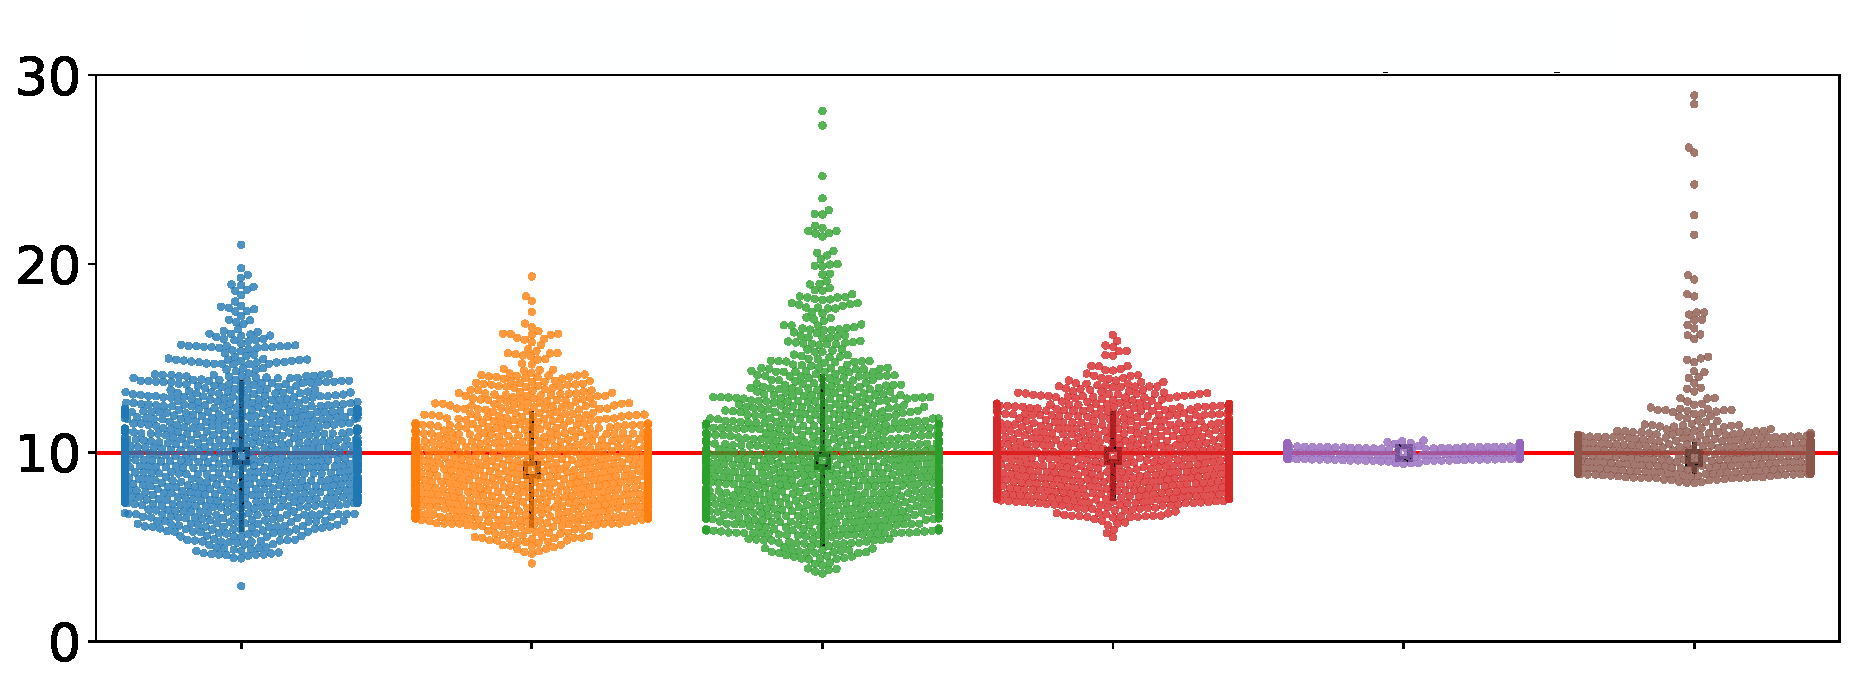
\includegraphics[width= \linewidth]{pics/boxplot_two_gaussian_dim_5.pdf}
    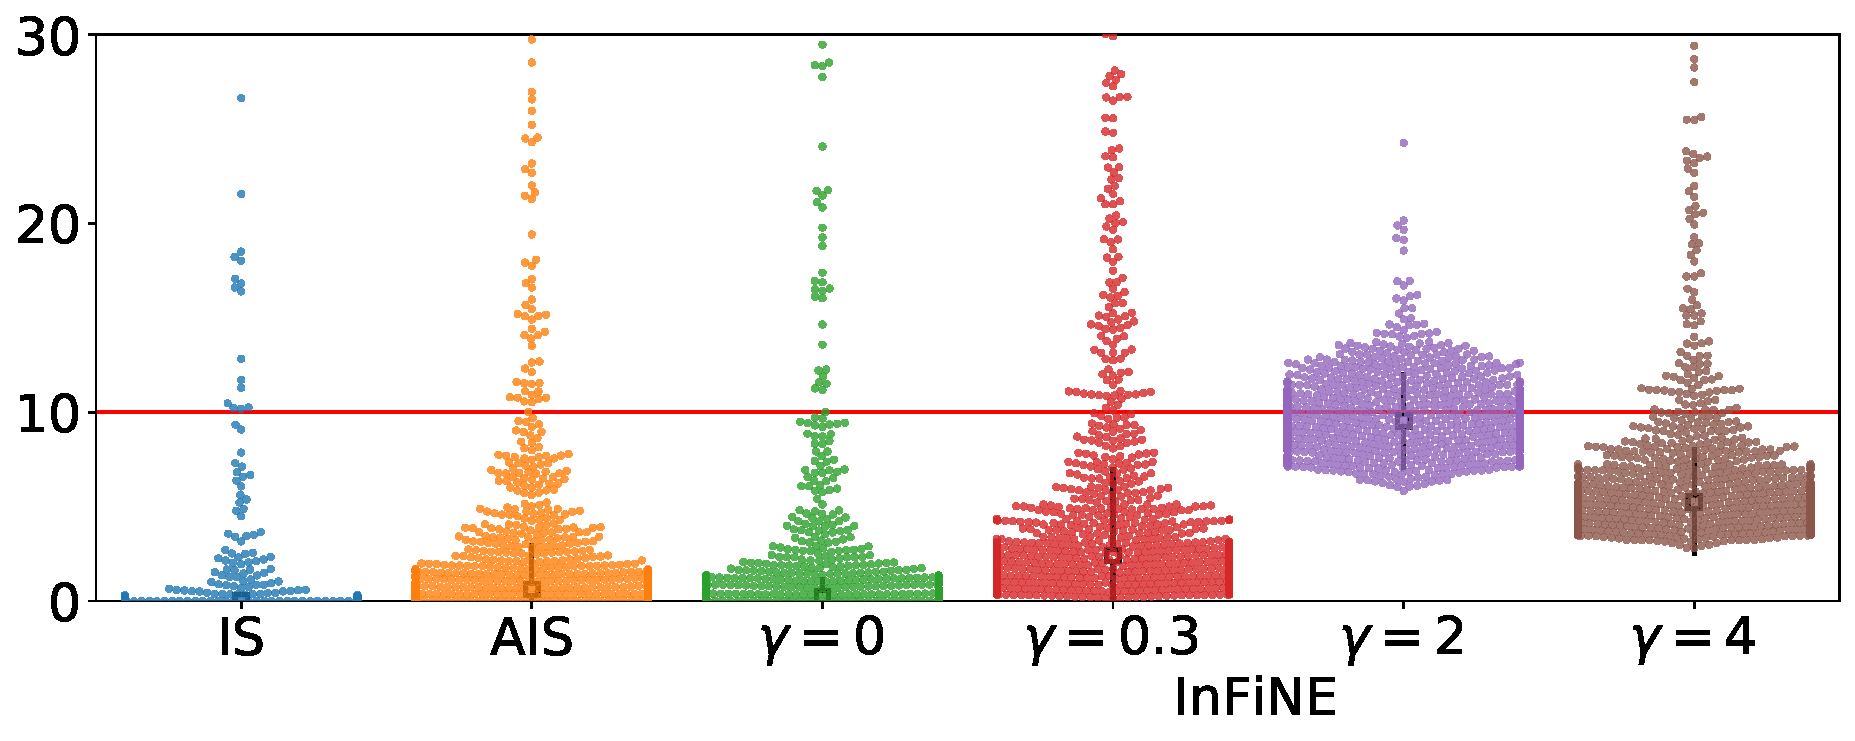
\includegraphics[width= \linewidth]{pics/boxplot_two_gaussian_dim_10.pdf}
    \caption{1000 independent estimations of the normalizing constant for each algorithm in the toy example:  a mixture of two Gaussian distributions, in dimension 5 (top) and 10 (bottom). The true value is $Z=10$ (red line). The figure displays the median (square) and the interquartile range (solid lines) in each case.}
    \label{fig:simple_gauss}
\end{figure}
We focus here on the impact of the damping factor $\gamma$ on the $\IFIS$ estimations.
\xian{check this is the case}
Further investigation on the stepsize $h$ and of the mass matrix $\mass$  are given in the supplementary material.

The number of steps $K$ is  a proxy of our computational budget (\ie~the number of times our transformation is applied). The mass matrix $\mass$ is chosen as the inverse of the covariance of the individual component of the mixture. Further tuning on this matrix is discussed in the supplementary material.
A first intuition on the role of $\gamma$ is shown in \Cref{fig:toy_example_posterior}. If $\gamma \ll 1$, then the trajectories are almost Hamiltonian, in which case we cannot easily explore all modes. On the other hand, if $\gamma \gg 1 $,  then trajectories are most often attracted by the ``closest'' mode. The resulting trade-off is easily observed on \Cref{fig:simple_gauss}, which displays the distribution of the different estimators.
%We present four examples of trajectories with different values for the damping factor $\gamma$. The performance of the associated estimators are displayed in \Cref{fig:simple_gauss}. %The target distribution here is a mixture of 2 $d$-dimensional concentrated Gaussians (diagonal covariance $\sigma^2 = 0.02$ ),
%\[
%p(z) = \tfrac{1}{2}(\Normal(y;-\mathbf{u}_d, \sigma^2\Id) +  \Normal(y;\mathbf{u}_d, \sigma^2\Id))\eqsp,
%\]
%where $\mathbf{u}_d$ is the $d$ dimensional vector with all coordinates set to 1.
%We choose $\rho$ to be a $d$-dimensional centered Gaussian, with diagonal covariance $\sigma^2_\rho \Id$, $\sigma^2_\rho=10$. We choose $d=10$ in our experiments.


The IS estimator is run with $4 \cdot 10^5$ samples.
For the \IFIS\ estimator, the number of samples is $N = 2 \cdot 10^4$ and the trajectory length is $K=20$. The stepsize is set to $h= 0.1$ for the conformal symplectic integrator.
The number of levels for AIS in the annealing schedule of AIS is set to $200$. At each intermediate temperature, an iteration of HMC is performed with 3 leapfrog steps (the size of leapfrog step is also set to 0.1).
The number of gradient computations is therefore equal to $4 \cdot 10^5$ for \IFIS\ and $6 \cdot 10^6$ for AIS, which is therefore 10 times more costly.

We further emphasize how the \IFIS\ estimator compares favorably to the AIS estimator albeit requiring a smaller computational budget.
\begin{figure}[!ht]
    \centering
    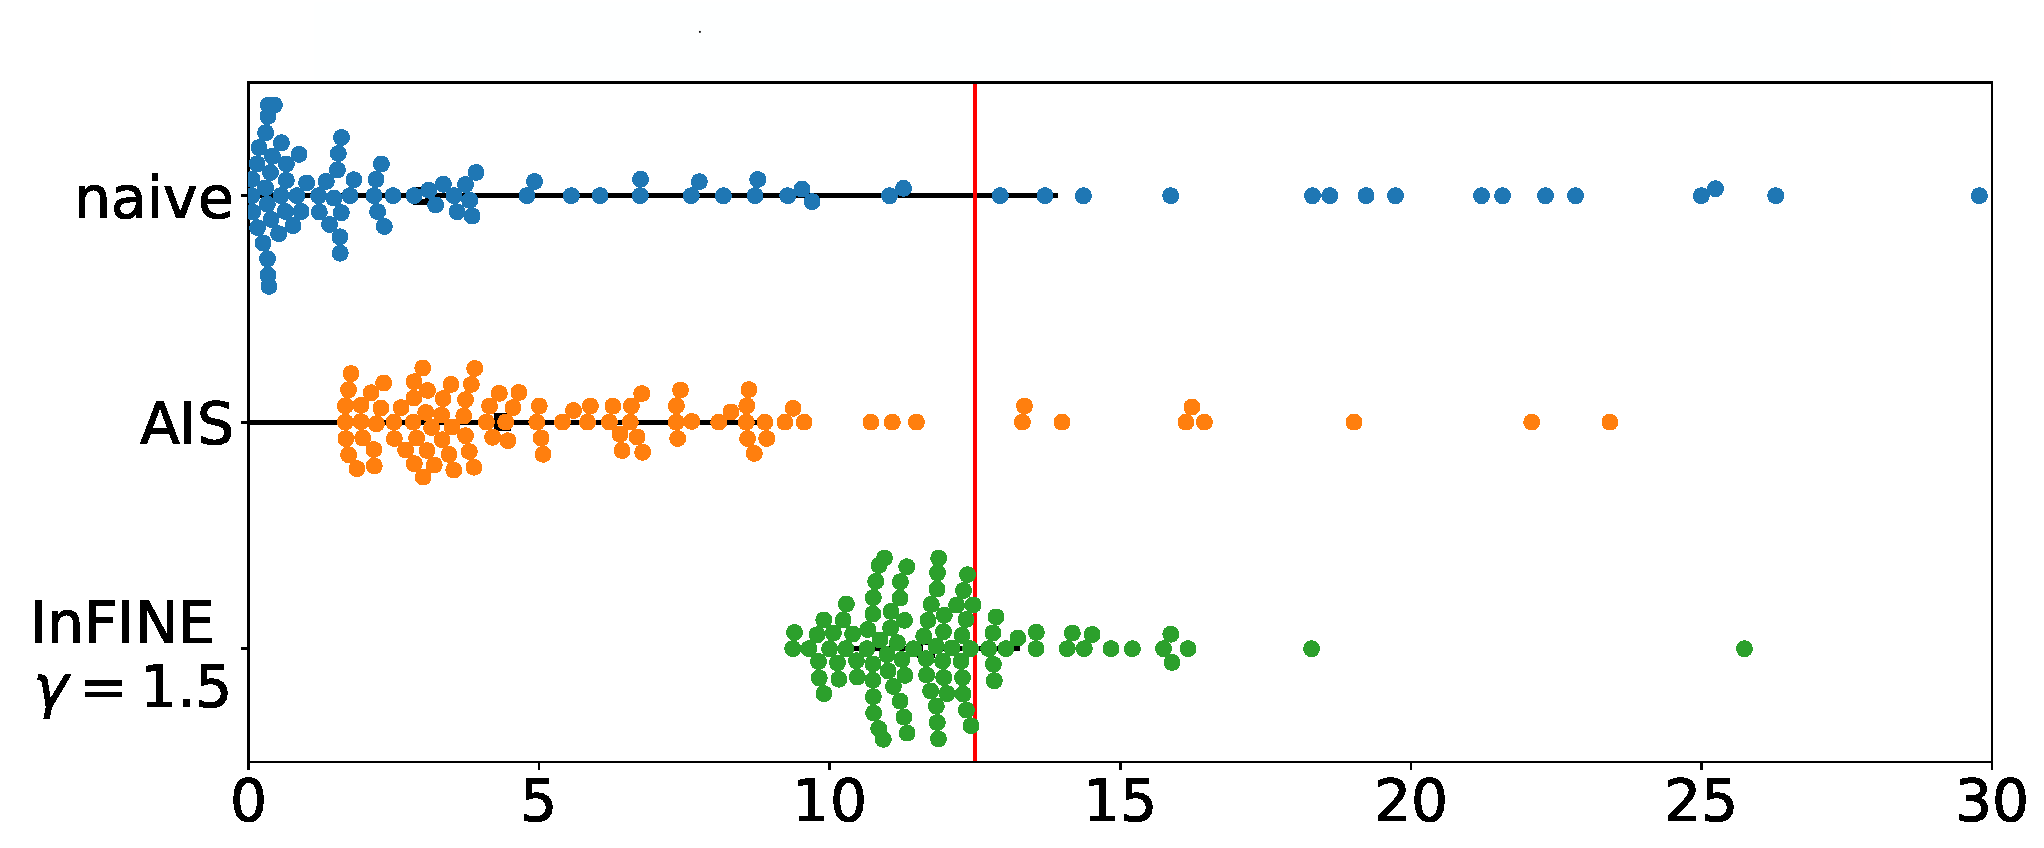
\includegraphics[width= 1.\linewidth]{pics/boxplot_dim10.pdf}
%        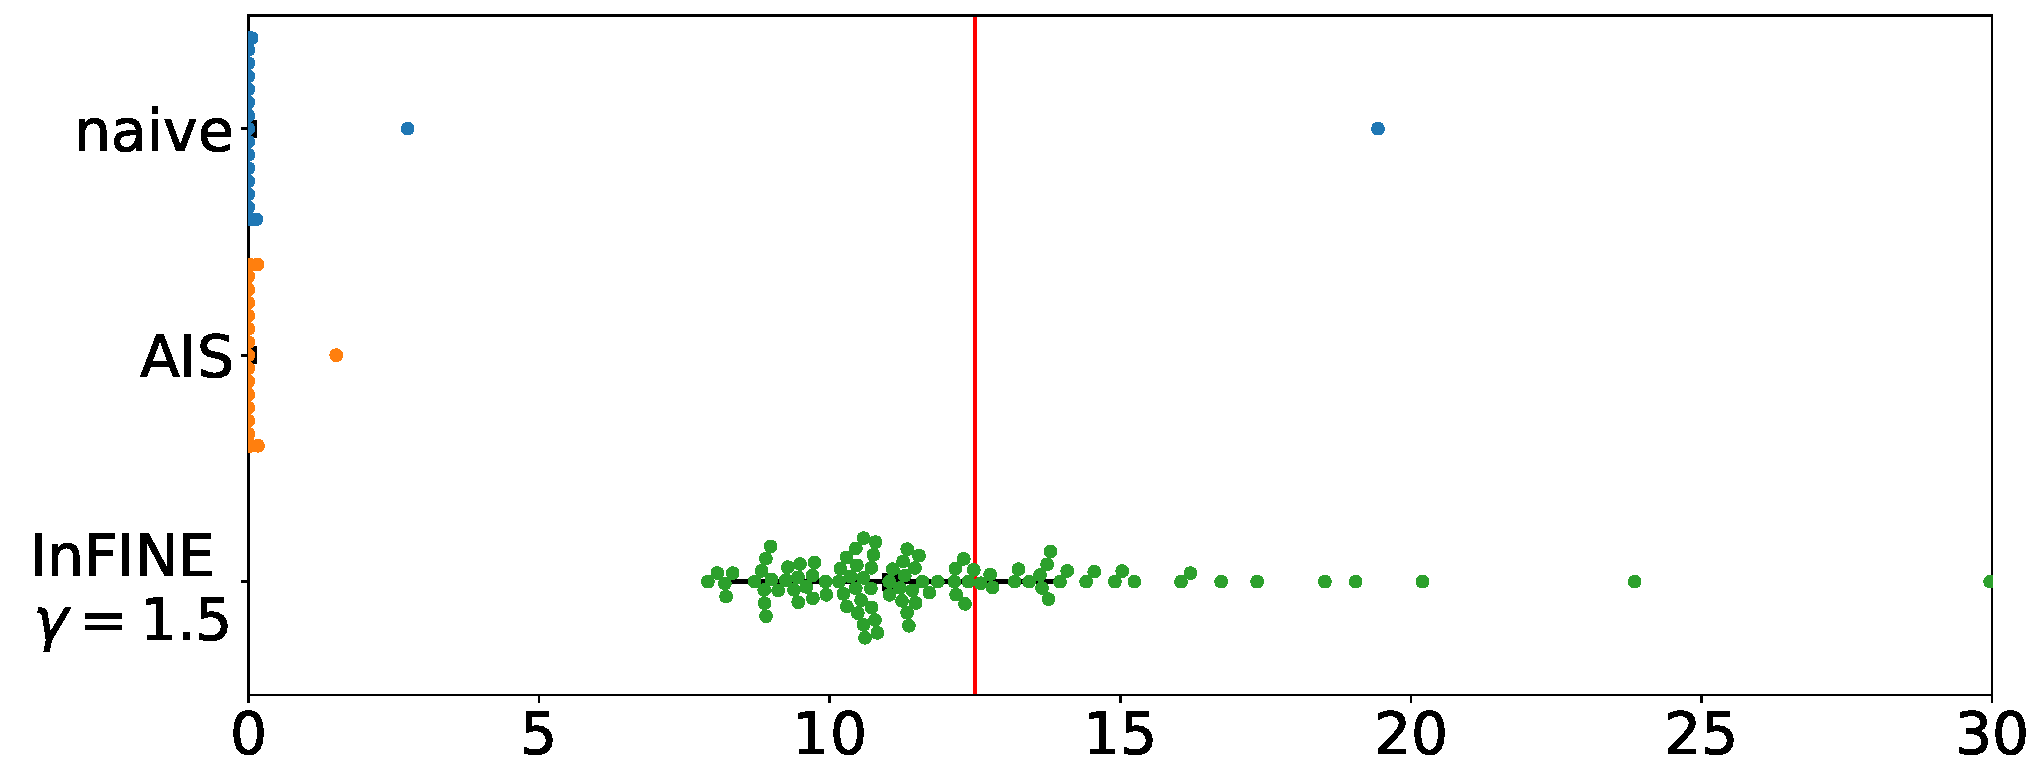
\includegraphics[width= 0.9\linewidth]{pics/boxplot_dim15.pdf}
        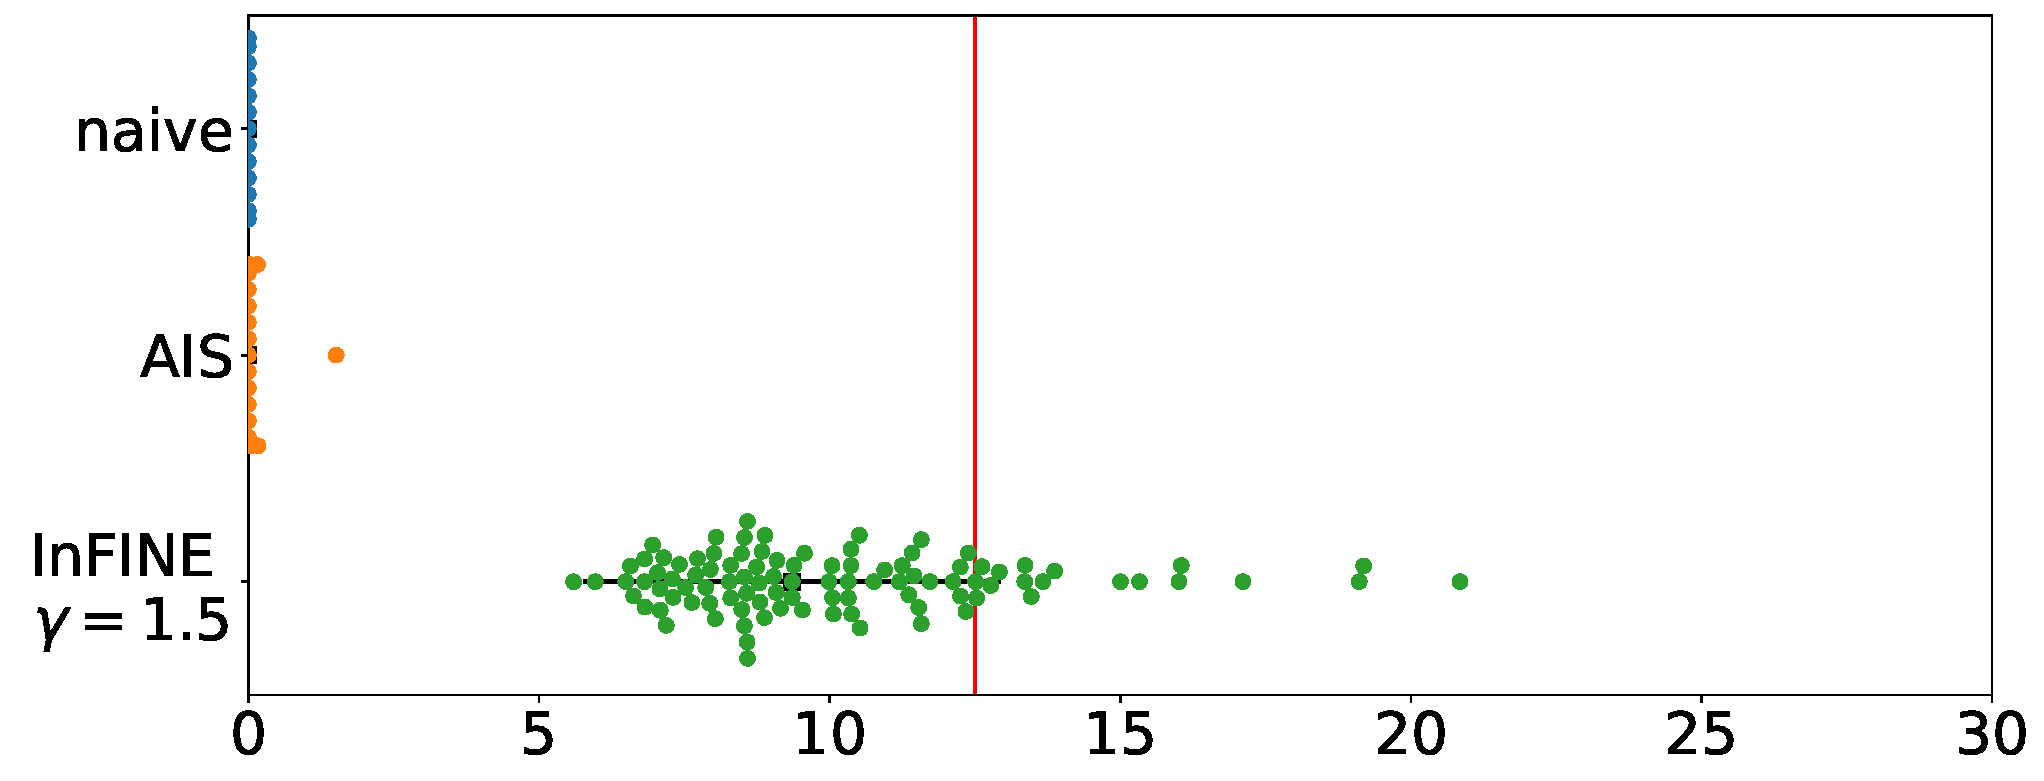
\includegraphics[width= 1.\linewidth]{pics/boxplot_dim20.pdf}
    \caption{$100$ independent estimations of the normalizing constant of the Gaussian mixture with 25 components in dimension 10 (top) and 20 (bottom) for each algorithm. The true value is $Z=12.5$ (red line).}
    \label{fig:25_gauss}
\end{figure}

The results for the 25-component Gaussian mixture are displayed in \Cref{fig:25_gauss}. In high dimension, the vanilla IS estimator unsurprisingly fails, since importance weighted estimates have notoriously poor scaling properties w.r.t. dimension. While AIS predictably improves upon vanilla IS, its performances are rather unsatisfactory, the estimator showing a very large variance. Regardless of the dimension $d$, the \IFIS\ estimator  is better behaved than the AIS estimator, although the computational burden for \IFIS\ is 10 times smaller.
\begin{comment}
\begin{table}[]
\caption{Results for the estimation of the normalizing constant in the toy example:  a mixture of two peaked Gaussians, in dimension 5. The true value is $Z=1$.}
\label{tab:simple_gaussian_est}
\begin{tabular}{c|c|c|}
\cline{2-3}
                                                 & Mean & Standard deviation \\ \hline
\multicolumn{1}{|c|}{IS estimate}                &    $6\cdot10^{-5}$  &           $6\cdot10^{-4}$         \\ \hline
\multicolumn{1}{|l|}{AIS estimate}               &  $3\cdot10^{-3}$    &    $2\cdot10^{-2}$                \\ \hline
\multicolumn{1}{|l|}{$\IFIS$ - $\gamma=0$}   &   $0.49$   &      4.9              \\ \hline
\multicolumn{1}{|l|}{$\IFIS$ - $\gamma=1$} &  $0.45$    &          2.5          \\ \hline
\multicolumn{1}{|l|}{$\IFIS$ - $\gamma=3$}   &   0.93   &   0.31                 \\ \hline
\multicolumn{1}{|l|}{$\IFIS$ - $\gamma=6$}   &  1.0    &        0.64            \\ \hline
\end{tabular}
\end{table}
\end{comment}
\subsection{MCMC experiments}
\label{subsec:mcmc_exp}
We focus here on sampling of the 25 Gaussian mixture example introduced in \Cref{subsec:estim_constant}. The dimension is set to $d=40$  and all the mixture components have diagonal covariances  $0.01 \Id_d$.
We compare the \InFiNE\ MCMC sampler with dependent proposals,
the No-U-Turn Sampler implemented with Pyro library \cite{bingham2019pyro},
and the ISIR scheme \cite{andrieu2010particle, andrieu2018uniform}, with correlated proposal.

For the \InFiNE\ MCMC, the number of particles is set to $N=10$, the length of trajectory is $K=10$, the stepsize of the conformal integrator is $h=0.1$, the mass matrix is diagonal with diagonal elements equal to 100. The proposal distribution is zero-mean Gaussian with diagonal covariance $5 \Id_d$. We use the proposal kernels $r_i$ defined in \eqref{eq:condition-kernel} with a random walk Metropolis kernel $m$ with zero-mean Gaussian increment distribution and covariance $0.01 \Id$.
For the iterated ISIR, we use the same number of proposals $N=10$,  proposal distribution $\proposal$ and proposal kernels $r_i$ as for \IFIS.  For NUTS, we use the default parameter (the mass matrix and stepsizes are adapted).

In \Cref{fig:25_gauss_mcmc}, the scatter plot of the first two components of the output is displayed. To make a fair comparison, we use the same wall clock time for all three algorithms. The number of iterations for CISIR, \IFIS, and NUTS are $n= 4\cdot 10^6$, $n= 4 \cdot 10^5$, and $n= 5 \cdot 10^5$, respectively.
\begin{figure}[!ht]
    \centering
    \begin{tabular}{cc}
      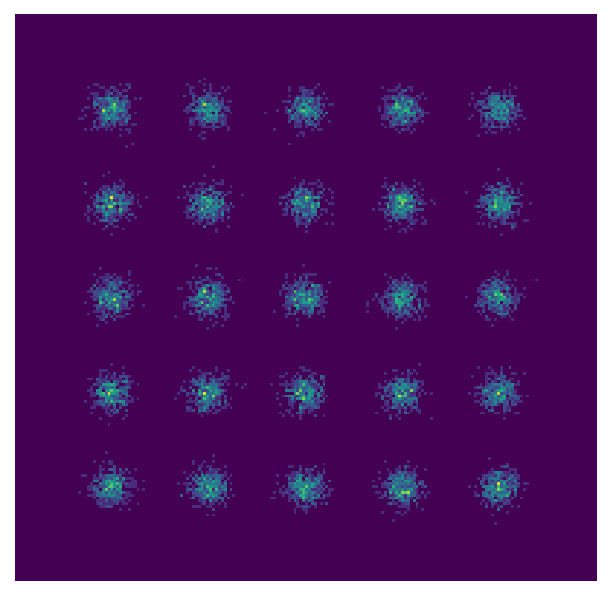
\includegraphics[width = .4\linewidth]{pics/histogram_true.pdf}
      &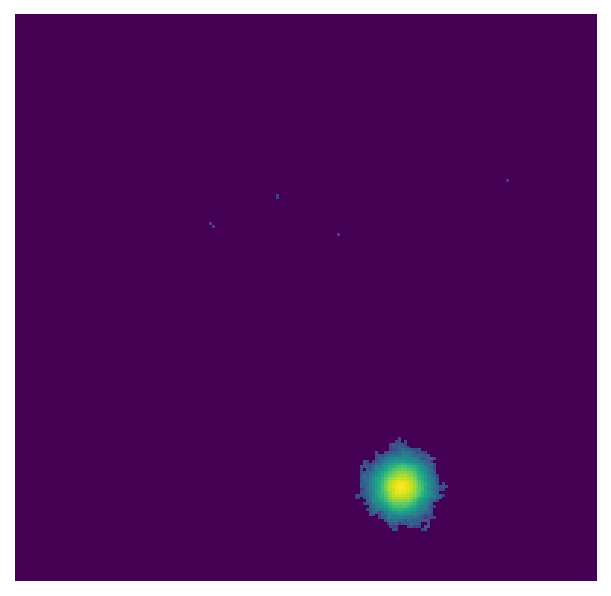
\includegraphics[width = .4\linewidth]{pics/histogram_isir.pdf}  \\
       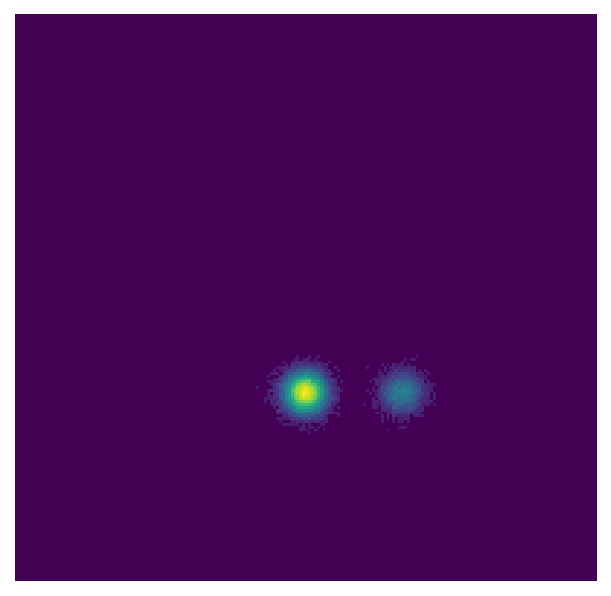
\includegraphics[width = .4\linewidth]{pics/histogram_nuts.pdf}
       &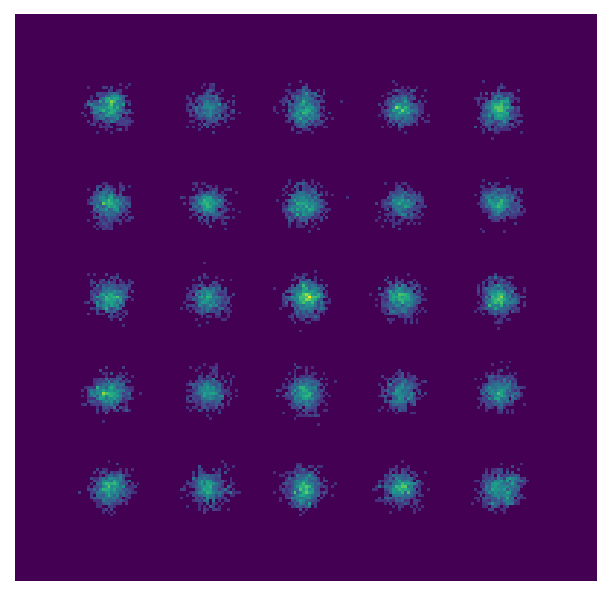
\includegraphics[width = .4\linewidth]{pics/histogram_infine.pdf}
    \end{tabular}
    \caption{Empirical 2-D histogram of the 10,000 samples of different algorithms targeting the mixture of 25 Gaussian distributions. Top row, from left to right: samples from the target distribution, correlated ISIR samples. Bottom row: NUTS samples, \InFiNE\ samples.}
    \label{fig:25_gauss_mcmc}
\end{figure}
\begin{table*}[!t]
\centering
\caption{Negative Log Likelihood estimates for VAE models for different latent space dimensions.}
\label{tab:vae_results2}
\begin{tabular}{c|c|c||c|c||c|c||c|c|}
\cline{2-9}
 & \multicolumn{2}{c||}{$d = 4$} & \multicolumn{2}{c||}{$d = 8$} & \multicolumn{2}{c||}{$d = 16$} & \multicolumn{2}{c|}{$d = 50$} \\ \hline
\multicolumn{1}{|c|}{model} & IS & \InFiNE  & IS & \InFiNE& IS  & \InFiNE & IS & \InFiNE \\ \hline
\multicolumn{1}{|c|}{VAE} & $115.01$&$113.49$&$97.96$&$97.64$&$90.52$&$90.42$&$88.22$&$88.36$\\ %\hline
\multicolumn{1}{|c|}{IWAE, $N=5$} & $113.33$&$111.83$&$97.19$&$96.61$&$89.34$&$89.05$&$87.49$&$87.27$ \\ %\hline
\multicolumn{1}{|c|}{IWAE, $N=30$} & $111.92$&$110.36$&$96.81$&$95.94$&$88.99$&$88.64$&$86.97$&$86.93$ \\ \hline
\multicolumn{1}{|c|}{\InFiNE\ VAE, $K=3$} & $109.14$&$107.47$&$94.50$&$94.26$&$89.03$&$88.92$&$88.14$&$88.16$ \\ %\hline
\multicolumn{1}{|c|}{\InFiNE\ VAE, $K=10$} & $110.02$&$107.90$&$94.63$&$94.22$&$89.71$&$88.68$&$88.25$&$86.95$ \\ \hline
\end{tabular}
\end{table*}

\subsection{VAE experiments}
\label{subsec:vae_experiments}
 Following \Cref{sec:extensions}, we propose numerical experiments to illustrate the relevance of  \IFIS\ in the context of VAEs. We build \IFIS\ VAE by optimizing directly the ELBO \eqref{eq:infine_elbo-alt} with respect to the parameters $(\theta, \phi)$ with a single trajectory. In practice, extending a standard VAE implementation with \IFIS\ is straightforward: after sampling the initial position $q$ from the encoder distribution $q_\phi(\cdot\mid x)$, an initial moment $p$ is sampled. The trajectory is then computed, followed by the weights and the ELBO.
The \textit{reparameterization trick} \cite{kingma:welling:2013} is used in a similar fashion as the VAE to ensure full differentiability of the whole architecture, enabling the optimization of all parameters. A full specification of the algorithm is provided in \Cref{subsec:vae_algo}.

We follow the experimental setting of \cite{burda:grosse:2015}, using the MNIST dataset. Additional experiments on the FashionMNIST dataset are given in \Cref{supsec:vae_exps}. We compare our \IFIS\ VAE with a classical VAE, and IWAE (with $N=5$ and $N=30$ samples).
For each setting, we use exactly the same architecture for the encoder and decoder, resulting in the same number of parameters. We followed as much as possible the implementation details (architecture and optimizer) detailed in \cite{burda:grosse:2015}. All models are trained during 200 epochs.


\paragraph{Estimating the loglikelihood}
After training, VAEs are classically evaluated by computing an estimate of their negative loglikelihood (NLL) using either IS, the IWAE bound, or AIS   \cite{wu:burda:grosse:2016}.
We first show here how $\IFIS$ competes with those methods for evaluating the NLL of VAEs.
Note that the methods for evaluating VAEs always define a lower bound of the true likelihood \eqref{eq:elbo}. We can thus compare two evaluation methods if one consistently gives lower NLL estimates.
\Cref{tab:vae_results2} gives the NLL estimate for the different models (associated with a different dimension $d$ of the latent variable). %The NLL is estimated here either using IS or \InFiNE.
In both cases, the importance distribution is  $q_\phi(\cdot\mid x)$.  We set up the \InFiNE\ estimator with a trajectory of length of $K=10$, $h= 0.1$ and $\gamma=2.5$ parameters.
The \InFiNE\ estimator consistently gives better estimates than the classical IS estimator.
%With this choice of parameters, the difference is clearer in small dimensions. 
%The objective here is not to derive state-of-the-art results but more to demonstrate the efficiency of our estimator, even without a thorough fine-tuning of all parameters.
%This can be understood as the \InFiNE is more robust to its hyperparameters in smaller dimensions.



\paragraph{Comparison of the different VAEs}
 Table~\ref{tab:vae_results2} displays the estimated NLL of all models provided by IS and the \InFiNE\ method. It is interesting to note here again that \InFiNE\ improves the training of the VAE when the dimension of the latent space is small to moderate. The relative improvement of \InFiNE\ decreases when the dimension of the latent space increases, most likely because the mean-field variational distribution is accurate enough in such cases  (this is at least the case for the MNIST dataset).
\InFiNE\ VAE has a better NLL than the VAE across all latent dimensions considered. %Moreover, it proves more efficient than IWAE again when latent dimension is small, but this advantage reduces when dimension of the latent space increases.

The results displayed in this section provide many insights for future research. Improving the NLL estimate in higher dimensions  can be linked to the \InFiNE\ hyperparameter tuning, which becomes crucial when the dimension increases. The optimal scaling of these hyperparameters remains an open (and challenging) problem left for future research as we aim here at highlighting the applicability  of \InFiNE\ in various contexts.   %This proves however that \InFiNE\ is well suited to design through optimization paths an efficient VAE.
Also, we have considered only the case $N=1$. It is expected that extension to $N > 1$ (similar to IWAE) will further improve the results.
\clearpage
%\newpage

% \section*{Broader Impact}
% Sampling from complex target distributions and computing their normalizing constants has numerous applications in machine learning and statistics but also bioinformatics, computational chemistry, protein folding etc. Our work proposes novel methods to address such problems and has thus potential applications in many areas.

% The techniques presented have been implemented in *****, which is available online for the benefit of other scientists. The method relies entirely on the target density defined by the user and does not itself leverage biases in the data. This work does not present any foreseeable societal consequence.
\bibliographystyle{icml2021}
\bibliography{bibliography}




\end{document} 